\documentclass{report}
%%%%%%%%%%%%%%%%%%%%%%%%%%%%%%%%%
% PACKAGE IMPORTS
%%%%%%%%%%%%%%%%%%%%%%%%%%%%%%%%%


\usepackage[tmargin=2cm,rmargin=1in,lmargin=1in,margin=0.85in,bmargin=2cm,footskip=.2in]{geometry} % I woulld suggest dont play with the margin. It kind of ruins the contents page.
\usepackage{amsmath,amsfonts,amsthm,amssymb,mathtools}
\usepackage{bookmark}
\usepackage[inline]{enumitem}
\usepackage{cancel}
\usepackage{hyperref,theoremref}
\hypersetup{
	colorlinks=true, linkcolor=doc!80, urlcolor=doc!80, citecolor=mydefinitfr!80!black,
	bookmarksnumbered=true,
	bookmarksopen=true
}
\usepackage[most,many,breakable]{tcolorbox}
\usepackage{xcolor}
\usepackage{graphicx}
%\graphicspath{ {./images/} } %give your suitable image path
\usepackage{varwidth}
\usepackage{authblk}
\usepackage{nameref}
\usepackage{multicol,array,multirow}
\usepackage{tikz-cd}
\usepackage{cancel}
\usepackage{caption} 
\usepackage{pgfplots}
%\usepackage[Sonny]{fncychap}
\usepackage{mathpazo}
% Use the libertine package for the Libertine font
\usepackage{libertine}
\usepackage[libertine]{newtxmath}
\usepackage{mathrsfs} 
\usepackage{bbm}
\usepackage[ruled,vlined,linesnumbered]{algorithm2e}
\usepackage{fancyhdr}
\pagestyle{fancy}
\fancypagestyle{plain}{%
	\renewcommand{\headrulewidth}{0pt}%
	\fancyhf{}%
}
\fancyhead{}
\renewcommand{\headrulewidth}{1pt}
\fancyhead[LE]{\itshape\textsc{\nouppercase\rightmark}}
\fancyhead[RO]{\itshape\textsc\leftmark} % CO Centered Odd
\fancyfoot{}
\fancyhead[RE,LO]{\itshape Page \thepage}
\makeatletter
\renewcommand{\chaptermark}[1]{%
  \markboth{%
    \ifnum\c@secnumdepth>\m@ne
      \@chapapp\ {\thechapter} \ %
    \fi
  #1%
  }{}%
}
\def\sectionmark#1{%
    \markright {\MakeUppercase{%
      \ifnum \c@secnumdepth >\z@
        \thesection \ %
      \fi
      #1}}}
\makeatother

\DeclareMathOperator{\supp}{supp}
\DeclareMathOperator{\rk}{Rank}
\DeclareMathOperator{\conv}{Conv}

%%%%%%%%%%%%%%%%%%%%%%%%%%%%%%
% SELF MADE COLORS
%%%%%%%%%%%%%%%%%%%%%%%%%%%%%%

\usetikzlibrary{ shapes.geometric }
\usetikzlibrary{calc}
\usepackage{anyfontsize}
\definecolor{doc}{RGB}{0,60,110}
\definecolor{myg}{RGB}{56, 140, 70}
\definecolor{myb}{RGB}{45, 111, 177}
\definecolor{myr}{RGB}{199, 68, 64}
\definecolor{mybg}{HTML}{F2F2F9}
\definecolor{mytheorembg}{HTML}{F2F2F9}
\definecolor{mytheoremfr}{HTML}{00007B}
\definecolor{myexamplebg}{HTML}{F2FBF8}
\definecolor{myexamplefr}{HTML}{88D6D1}
\definecolor{myexampleti}{HTML}{2A7F7F}
\definecolor{mydefinitbg}{HTML}{E5E5FF}
\definecolor{mydefinitfr}{HTML}{3F3FA3}
\definecolor{notesgreen}{RGB}{0,162,0}
\definecolor{myp}{RGB}{197, 92, 212}
\definecolor{mygr}{HTML}{2C3338}
\definecolor{myred}{RGB}{127,0,0}
\definecolor{myyellow}{RGB}{169,121,69}
\definecolor{OrangeRed}{HTML}{ED135A}
\definecolor{Dandelion}{HTML}{FDBC42}
\definecolor{light-gray}{gray}{0.95}
\definecolor{Emerald}{HTML}{00A99D}
\definecolor{RoyalBlue}{HTML}{0071BC}

\renewcommand{\qed}{\ensuremath{\blacksquare}}



%%%%%%%%%%%%%%%%%%%%%%%%%%%%
% TCOLORBOX SETUPS
%%%%%%%%%%%%%%%%%%%%%%%%%%%%

\setlength{\parindent}{1cm}
%================================
% THEOREM BOX
%================================

\tcbuselibrary{theorems,skins,hooks}
\newtcbtheorem[number within=section]{Theorem}{Theorem}
{%
	enhanced,
	breakable,
	colback = mytheorembg,
	frame hidden,
	boxrule = 0sp,
	borderline west = {2pt}{0pt}{mytheoremfr},
	sharp corners,
	detach title,
	before upper = \tcbtitle\par\smallskip,
	coltitle = mytheoremfr,
	fonttitle = \bfseries\sffamily,
	description font = \mdseries,
	separator sign none,
	segmentation style={solid, mytheoremfr},
}
{th}

\tcbuselibrary{theorems,skins,hooks}
\newtcbtheorem[number within=chapter]{theorem}{Theorem}
{%
	enhanced,
	breakable,
	colback = mytheorembg,
	frame hidden,
	boxrule = 0sp,
	borderline west = {2pt}{0pt}{mytheoremfr},
	sharp corners,
	detach title,
	before upper = \tcbtitle\par\smallskip,
	coltitle = mytheoremfr,
	fonttitle = \bfseries\sffamily,
	description font = \mdseries,
	separator sign none,
	segmentation style={solid, mytheoremfr},
}
{th}


\tcbuselibrary{theorems,skins,hooks}
\newtcolorbox{Theoremcon}
{%
	enhanced
	,breakable
	,colback = mytheorembg
	,frame hidden
	,boxrule = 0sp
	,borderline west = {2pt}{0pt}{mytheoremfr}
	,sharp corners
	,description font = \mdseries
	,separator sign none
}


%================================
% Corollery
%================================
\tcbuselibrary{theorems,skins,hooks}
\newtcbtheorem[use counter from=Theorem, number within=section]{corolary}{Corollary}
{%
	enhanced
	,breakable
	,colback = myp!10
	,frame hidden
	,boxrule = 0sp
	,borderline west = {2pt}{0pt}{myp!60!black}
	,sharp corners
	,detach title
	,before upper = \tcbtitle\par\smallskip
	,coltitle = myp!60!black
	,fonttitle = \bfseries\sffamily
	,description font = \mdseries
	,separator sign none
	,segmentation style={solid, myp!85!black}
%	enhanced
%	,breakable
%	,colback = mytheorembg
%	,frame hidden
%	,boxrule = 0sp
%	,borderline west = {2pt}{0pt}{mytheoremfr}
%	,sharp corners
%	,detach title
%	,before upper = \tcbtitle\par\smallskip
%	,coltitle = mytheoremfr
%	,fonttitle = \bfseries\sffamily
%	,description font = \mdseries
%	,separator sign none
%	,segmentation style={solid, mytheoremfr}
}
{th}
\tcbuselibrary{theorems,skins,hooks}
\newtcbtheorem[use counter from=Theorem, number within=chapter]{corollary}{Corollary}
{%
	enhanced
	,breakable
	,colback = mytheorembg
	,frame hidden
	,boxrule = 0sp
	,borderline west = {2pt}{0pt}{mytheoremfr}
	,sharp corners
	,detach title
	,before upper = \tcbtitle\par\smallskip
	,coltitle = mytheoremfr
	,fonttitle = \bfseries\sffamily
	,description font = \mdseries
	,separator sign none
	,segmentation style={solid, mytheoremfr}
}
{th}

%================================
% LEMMA
%================================

\tcbuselibrary{theorems,skins,hooks}
\newtcbtheorem[use counter from=Theorem, number within=section]{lemma}{Lemma}
{%
	enhanced
	,breakable
	,colback = myg!10
	,frame hidden
	,boxrule = 0sp
	,borderline west = {2pt}{0pt}{myg}
	,sharp corners
	,detach title
	,before upper = \tcbtitle\par\smallskip
	,coltitle = myg!85!black
	,fonttitle = \bfseries\sffamily
	,description font = \mdseries
	,separator sign none
	,segmentation style={solid, myg!85!black}
}
{th}


\newtcbtheorem[use counter from=theorem, number within=chapter]{Lemma}{Lemma}
{%
	enhanced
	,breakable
	,colback = myg!10
	,frame hidden
	,boxrule = 0sp
	,borderline west = {2pt}{0pt}{myg}
	,sharp corners
	,detach title
	,before upper = \tcbtitle\par\smallskip
	,coltitle = myg!85!black
	,fonttitle = \bfseries\sffamily
	,description font = \mdseries
	,separator sign none
	,segmentation style={solid, myg!85!black}
}
{th}

%================================
% CLAIM
%================================

\tcbuselibrary{theorems,skins,hooks}
\newtcbtheorem[number within=section]{claim}{Claim}
{%
	enhanced
	,breakable
	,colback = myg!10
	,frame hidden
	,boxrule = 0sp
	,borderline west = {2pt}{0pt}{myg}
	,sharp corners
	,detach title
	,before upper = \tcbtitle\par\smallskip
	,coltitle = myg!85!black
	,fonttitle = \bfseries\sffamily
	,description font = \mdseries
	,separator sign none
	,segmentation style={solid, myg!85!black}
}
{th}


\newtcbtheorem[number within=chapter]{Claim}{Claim}
{%
	enhanced
	,breakable
	,colback = myg!10
	,frame hidden
	,boxrule = 0sp
	,borderline west = {2pt}{0pt}{myg}
	,sharp corners
	,detach title
	,before upper = \tcbtitle\par\smallskip
	,coltitle = myg!85!black
	,fonttitle = \bfseries\sffamily
	,description font = \mdseries
	,separator sign none
	,segmentation style={solid, myg!85!black}
}
{th}

%================================
% EXAMPLE BOX
%================================

\newtcbtheorem[number within=section]{Example}{Example}
{%
	colback = myexamplebg
	,breakable
	,colframe = myexamplefr
	,coltitle = myexampleti
	,boxrule = 1pt
	,sharp corners
	,detach title
	,before upper=\tcbtitle\par\smallskip
	,fonttitle = \bfseries
	,description font = \mdseries
	,separator sign none
	,description delimiters parenthesis
}
{ex}

\newtcbtheorem[number within=chapter]{example}{Example}
{%
	colback = myexamplebg
	,breakable
	,colframe = myexamplefr
	,coltitle = myexampleti
	,boxrule = 1pt
	,sharp corners
	,detach title
	,before upper=\tcbtitle\par\smallskip
	,fonttitle = \bfseries
	,description font = \mdseries
	,separator sign none
	,description delimiters parenthesis
}
{ex}

%================================
% DEFINITION BOX
%================================

\newtcbtheorem[number within=section]{Definition}{Definition}{enhanced,
	before skip=2mm,after skip=2mm, colback=red!5,colframe=red!80!black,boxrule=0.5mm,
	attach boxed title to top left={xshift=1cm,yshift*=1mm-\tcboxedtitleheight}, varwidth boxed title*=-3cm,colbacktitle=red!75!black,
	boxed title style={frame code={
			\path[fill=tcbcolback]
			([yshift=-1mm,xshift=-1mm]frame.north west)
			arc[start angle=0,end angle=180,radius=1mm]
			([yshift=-1mm,xshift=1mm]frame.north east)
			arc[start angle=180,end angle=0,radius=1mm];
			\path[left color=tcbcolback!60!black,right color=tcbcolback!60!black,
			middle color=tcbcolback!80!black]
			([xshift=-2mm]frame.north west) -- ([xshift=2mm]frame.north east)
			[rounded corners=1mm]-- ([xshift=1mm,yshift=-1mm]frame.north east)
			-- (frame.south east) -- (frame.south west)
			-- ([xshift=-1mm,yshift=-1mm]frame.north west)
			[sharp corners]-- cycle;
		},interior engine=empty,
	},
	fonttitle=\bfseries,
	title={#2},#1}{def}
\newtcbtheorem[number within=chapter]{definition}{Definition}{enhanced,
	before skip=2mm,after skip=2mm, colback=red!5,colframe=red!80!black,boxrule=0.5mm,
	attach boxed title to top left={xshift=1cm,yshift*=1mm-\tcboxedtitleheight}, varwidth boxed title*=-3cm, colbacktitle=red!75!black,
	boxed title style={frame code={
			\path[fill=red!75!black]
			([yshift=-1mm,xshift=-1mm]frame.north west)
			arc[start angle=0,end angle=180,radius=1mm]
			([yshift=-1mm,xshift=1mm]frame.north east)
			arc[start angle=180,end angle=0,radius=1mm];
			\path[left color=tcbcolback!60!black,right color=tcbcolback!60!black,
			middle color=tcbcolback!80!black]
			([xshift=-2mm]frame.north west) -- ([xshift=2mm]frame.north east)
			[rounded corners=1mm]-- ([xshift=1mm,yshift=-1mm]frame.north east)
			-- (frame.south east) -- (frame.south west)
			-- ([xshift=-1mm,yshift=-1mm]frame.north west)
			[sharp corners]-- cycle;
		},interior engine=empty,
	},
	fonttitle=\bfseries,
	title={#2},#1}{def}


%================================
% OPEN QUESTION BOX
%================================

\newtcbtheorem[number within=section]{open}{Open Question}{enhanced,
	before skip=2mm,after skip=2mm, colback=myp!5,colframe=myp!80!black,boxrule=0.5mm,
	attach boxed title to top left={xshift=1cm,yshift*=1mm-\tcboxedtitleheight}, varwidth boxed title*=-3cm, colbacktitle=myp!75!black,
	boxed title style={frame code={
			\path[fill=tcbcolback]
			([yshift=-1mm,xshift=-1mm]frame.north west)
			arc[start angle=0,end angle=180,radius=1mm]
			([yshift=-1mm,xshift=1mm]frame.north east)
			arc[start angle=180,end angle=0,radius=1mm];
			\path[left color=tcbcolback!60!black,right color=tcbcolback!60!black,
			middle color=tcbcolback!80!black]
			([xshift=-2mm]frame.north west) -- ([xshift=2mm]frame.north east)
			[rounded corners=1mm]-- ([xshift=1mm,yshift=-1mm]frame.north east)
			-- (frame.south east) -- (frame.south west)
			-- ([xshift=-1mm,yshift=-1mm]frame.north west)
			[sharp corners]-- cycle;
		},interior engine=empty,
	},
	fonttitle=\bfseries,
	title={#2},#1}{def}
\newtcbtheorem[number within=chapter]{Open}{Open Question}{enhanced,
	before skip=2mm,after skip=2mm, colback=myp!5,colframe=myp!80!black,boxrule=0.5mm,
	attach boxed title to top left={xshift=1cm,yshift*=1mm-\tcboxedtitleheight}, varwidth boxed title*=-3cm, colbacktitle=myp!75!black,
	boxed title style={frame code={
			\path[fill=tcbcolback]
			([yshift=-1mm,xshift=-1mm]frame.north west)
			arc[start angle=0,end angle=180,radius=1mm]
			([yshift=-1mm,xshift=1mm]frame.north east)
			arc[start angle=180,end angle=0,radius=1mm];
			\path[left color=tcbcolback!60!black,right color=tcbcolback!60!black,
			middle color=tcbcolback!80!black]
			([xshift=-2mm]frame.north west) -- ([xshift=2mm]frame.north east)
			[rounded corners=1mm]-- ([xshift=1mm,yshift=-1mm]frame.north east)
			-- (frame.south east) -- (frame.south west)
			-- ([xshift=-1mm,yshift=-1mm]frame.north west)
			[sharp corners]-- cycle;
		},interior engine=empty,
	},
	fonttitle=\bfseries,
	title={#2},#1}{def}



%================================
% EXERCISE BOX
%================================

\makeatletter
\newtcbtheorem[number within=chapter]{problem}{Problem}{enhanced,
	breakable,
	colback=white,
	colframe=myb!80!black,
	attach boxed title to top left={yshift*=-\tcboxedtitleheight},
	fonttitle=\bfseries,
	title={#2},
	boxed title size=title,
	boxed title style={%
		sharp corners,
		rounded corners=northwest,
		colback=tcbcolframe,
		boxrule=0pt,
	},
	underlay boxed title={%
		\path[fill=tcbcolframe] (title.south west)--(title.south east)
		to[out=0, in=180] ([xshift=5mm]title.east)--
		(title.center-|frame.east)
		[rounded corners=\kvtcb@arc] |-
		(frame.north) -| cycle;
	},
	#1
}{def}
\makeatother


%================================
% Question BOX
%================================


\makeatletter
\newtcbtheorem[number within=chapter]{question}{Question}{enhanced,
	breakable,
	colback=white,
	colframe=myb!80!black,
	attach boxed title to top left={yshift*=-\tcboxedtitleheight},
	fonttitle=\bfseries,
	title={#2},
	boxed title size=title,
	boxed title style={%
		sharp corners,
		rounded corners=northwest,
		colback=tcbcolframe,
		boxrule=0pt,
	},
	underlay boxed title={%
		\path[fill=tcbcolframe] (title.south west)--(title.south east)
		to[out=0, in=180] ([xshift=5mm]title.east)--
		(title.center-|frame.east)
		[rounded corners=\kvtcb@arc] |-
		(frame.north) -| cycle;
	},
	#1
}{qs}
\makeatother

\newtcbtheorem[number within=chapter]{wconc}{Wrong Concept}{
	breakable,
	enhanced,
	colback=white,
	colframe=myr,
	arc=0pt,
	outer arc=0pt,
	fonttitle=\bfseries\sffamily\large,
	colbacktitle=myr,
	attach boxed title to top left={},
	boxed title style={
		enhanced,
		skin=enhancedfirst jigsaw,
		arc=3pt,
		bottom=0pt,
		interior style={fill=myr}
	},
	#1
}{def}


%================================
% NOTE BOX (with customizable title)
%================================

\usetikzlibrary{arrows,calc,shadows.blur}
\tcbuselibrary{skins}
% I've redefined this to take a mandatory argument for the title
\newtcolorbox{note}[2][]{% % CHANGED: Now takes 2 arguments, second is for the title
	enhanced jigsaw,
	colback=gray!20!white,%
	colframe=gray!80!black,
	size=small,
	boxrule=1pt,
	title=\textbf{#2}, % CHANGED: Title is now set by the second argument
	halign title=flush center,
	coltitle=black,
	breakable,
	drop shadow=black!50!white,
	attach boxed title to top left={xshift=1cm,yshift=-\tcboxedtitleheight/2,yshifttext=-\tcboxedtitleheight/2},
	minipage boxed title=1.5cm,
	boxed title style={%
		colback=white,
		size=fbox,
		boxrule=1pt,
		boxsep=2pt,
		underlay={%
			\coordinate (dotA) at ($(interior.west) + (-0.5pt,0)$);
			\coordinate (dotB) at ($(interior.east) + (0.5pt,0)$);
			\begin{scope}
				\clip (interior.north west) rectangle ([xshift=3ex]interior.east);
				\filldraw [white, blur shadow={shadow opacity=60, shadow yshift=-.75ex}, rounded corners=2pt] (interior.north west) rectangle (interior.south east);
			\end{scope}
			\begin{scope}[gray!80!black]
				\fill (dotA) circle (2pt);
				\fill (dotB) circle (2pt);
			\end{scope}
		},
	},
	#1,
}

%================================
% Algorithm Problem Definition
%================================

\makeatletter
\usepackage{tabularx,environ}
\newcommand{\problemtitle}[1]{\gdef\@problemtitle{\scshape #1}}% Store problem title
\newcommand{\probleminput}[1]{\gdef\@probleminput{#1}}% Store problem input
\newcommand{\problemquestion}[1]{\gdef\@problemquestion{#1}}% Store problem question
\NewEnviron{algoprob}{
	\problemtitle{}\probleminput{}\problemquestion{}% Default input is empty
	\BODY% Parse input
	\par\addvspace{.5\baselineskip}
	\noindent
	\begin{tabularx}{\textwidth}{@{\hspace{\parindent}} l X c}
		\multicolumn{2}{@{\hspace{\parindent}}l}{\@problemtitle} \\% Title
		\textbf{Input:} & \@probleminput \\% Input
		\textbf{Question:} & \@problemquestion% Question
	\end{tabularx}
	\par\addvspace{.5\baselineskip}
}
\makeatother


%%%%%%%%%%%%%%%%%%%%%%%%%%%%%%
% SELF MADE COMMANDS
%%%%%%%%%%%%%%%%%%%%%%%%%%%%%%

%% The environments which are appears in pairs one of them is for the chapters which have sections whose environment name starts with small letter and the other is for chapters which do not have sections whose environment name starts with capital letter. In the short command for the latter I used the letter 'c' to represent it should be use if it is not under a section

%% Short commands for environments goes like this
%% \<command name>[<reference name>]{<heading>}{<description>}
%% For example in theorem for suppose Fundamental Theorem of Calculus i will write like this
%% \thm[ftc]{Fundamental Theorem of Calculus}{Theorem Statement}

\NewDocumentCommand{\EqM}{ m O{black} m}{%
	\tikz[remember picture, baseline, anchor=base] 
	\node[inner sep=0pt, outer sep=3pt, text=#2] (#1) {%
		\ensuremath{#3}%
	};    
}



\newcommand{\thm}[3][]{\begin{Theorem}{#2}{#1}#3\end{Theorem}}
\newcommand{\thmc}[3][]{\begin{theorem}{#2}{#1}#3\end{theorem}}
\newcommand{\cor}[3][]{\begin{corolary}{#2}{#1}#3\end{corolary}}
\newcommand{\corc}[3][]{\begin{corollary}{#2}{#1}#3\end{corollary}}
\newcommand{\lem}[3][]{\begin{lemma}{#2}{#1}#3\end{lemma}}
\newcommand{\clm}[3][]{\begin{claim}{#2}{#1}#3\end{claim}}
\newcommand{\wc}[3][]{\begin{wconc}{#2}{#1}\setlength{\parindent}{1cm}#3\end{wconc}}
\newcommand{\thmcon}[1]{\begin{Theoremcon}{#1}\end{Theoremcon}}
\newcommand{\ex}[3][]{\begin{Example}{#2}{#1}#3\end{Example}}
\newcommand{\exc}[3][]{\begin{example}{#2}{#1}#3\end{example}}
\newcommand{\dfn}[3][]{\begin{Definition}{#2}{#1}#3\end{Definition}}
\newcommand{\dfnc}[3][]{\begin{definition}{#2}{#1}#3\end{definition}}
\newcommand{\opn}[3][]{\begin{open}{#2}{#1}#3\end{open}}
\newcommand{\opnc}[3][]{\begin{Open}{#2}{#1}#3\end{Open}}
\newcommand{\pr}[3][]{\begin{problem}{#2}{#1}#3\end{problem}}





\newtheorem*{observation*}{Observation}
\newtheorem*{idea*}{Idea}
\newtheorem*{assumption*}{Assumption}
\newtheorem{observation}{Observation}
\newtheorem{fact}[observation]{Fact}
\newtheorem{assumption}{Assumption}[section]


\renewenvironment{proof}{\noindent{\it \textbf{Proof:}}\hspace*{1em}}{\hfill\qed\bigskip\\}
\newenvironment{proof-sketch}{\noindent{\it \bf Sketch of Proof:}\hspace*{1em}}{\hfill\qed\bigskip\\}
\newenvironment{proof-idea}{\noindent{\it \bf Proof Idea:}\hspace*{1em}}{\hfill\qed\bigskip\\}
\newenvironment{proof-of-theorem}[1]{\noindent{\it \bf Proof of \thmref{#1}:}\hspace*{1em}}{\hfill\qed\bigskip\\}
\newenvironment{proof-of-lemma}[1]{\noindent{\it \bf Proof of Lemma \lemref{#1}:}\hspace*{1em}}{\hfill\qed\bigskip\\}
\newenvironment{proof-of-corollary}[1]{\noindent{\it \bf Proof of \corrref{#1}:}\hspace*{1em}}{\hfill\qed\bigskip\\}
\newenvironment{proof-attempt}{\noindent{\it \bf Proof Attempt:}\hspace*{1em}}{\hfill\qed\bigskip\\}
\newenvironment{alternate-proof}[1][]{\noindent{\textit{\textbf{Alternate Proof }#1:}}\hspace*{1em}}{\hfill\qed\bigskip\\}
\newenvironment{proofof}[1]{\noindent{\bf Proof:}
	of #1:\hspace*{1em}}{\hfill\qed\bigskip\\}
\newenvironment{remark}{\noindent{\bf Remark:}\hspace*{1em}}{\bigskip\\}
\newenvironment{idea}{\noindent{\bf Idea: }}{\bigskip\\}



%% The proof environment actually multipurpose. For a proof many things actually play. Proof idea. Proof overview. Main pproof. Proof prerequisites etc. Thats why the first option uses the actual name of what exactly we are writing for the proof. It will go like this
%% Proof idea: \pf{Proof Idea}{content..}
%% Proof Overview: \pf{Proof Overview}{content..}
%% Proof : \pf{Proof}{content..}


%================================
% SELF MADE COMMANDS
%================================

% ... (other commands) ...

% UPDATED NOTE COMMAND
% Usage: \nt{Your Custom Title}{The content of the note...}
\newcommand{\nt}[2]{\begin{note}{#1}#2\end{note}}

% ... (rest of your preamble file) ...

\newcounter{mylabelcounter}



\makeatletter
\newcommand{\setword}[2]{%
	\phantomsection
	#1\def\@currentlabel{\unexpanded{#1}}\label{#2}%
}
\makeatother




\tikzset{
	symbol/.style={
		draw=none,
		every to/.append style={
			edge node={node [sloped, allow upside down, auto=false]{$#1$}}}
	}
}


%%%%%%%%%%%%%%%%%%%%%%%%%%%%%%%%%%%%%%%%%%%
% TABLE OF CONTENTS 1
%%%%%%%%%%%%%%%%%%%%%%%%%%%%%%%%%%%%%%%%%%%
%
%\usepackage{framed}
%\usepackage{titletoc}
%\usepackage{etoolbox}
%\usepackage{lmodern}
%
%
%\patchcmd{\tableofcontents}{\contentsname}{\sffamily\contentsname}{}{}
%
%\renewenvironment{leftbar}
%{\def\FrameCommand{\hspace{6em}%
%				{\color{myyellow}\vrule width 2pt depth 6pt}\hspace{1em}}%
%		\MakeFramed{\parshape 1 0cm \dimexpr\textwidth-6em\relax\FrameRestore}\vskip2pt%
%	}
%{\endMakeFramed}
%
%\titlecontents{chapter}
%[0em]{\vspace*{2\baselineskip}}
%{\parbox{4.5em}{%
%				\hfill\Huge\sffamily\bfseries\color{myred}\thecontentspage}%
%		\vspace*{-2.3\baselineskip}\leftbar\textsc{\small\chaptername~\thecontentslabel}\\\sffamily}
%{}{\endleftbar}
%\titlecontents{section}
%[8.4em]
%{\sffamily\contentslabel{3em}}{}{}
%{\hspace{0.5em}\nobreak\itshape\color{myred}\contentspage}
%\titlecontents{subsection}
%[8.4em]
%{\sffamily\contentslabel{3em}}{}{}  
%{\hspace{0.5em}\nobreak\itshape\color{myred}\contentspage}



%%%%%%%%%%%%%%%%%%%%%%%%%%%%%%%%%%%%%%%%%%%
% TABLE OF CONTENTS 2
%%%%%%%%%%%%%%%%%%%%%%%%%%%%%%%%%%%%%%%%%%%

\usepackage{tikz}
\usetikzlibrary{shapes, positioning}
\usepackage{titletoc,titlesec}
\contentsmargin{0cm}
\titlecontents{chapter}[3.7pc]
{\addvspace{30pt}%
	\begin{tikzpicture}[remember picture, overlay]%
		\draw[fill=doc!60,draw=doc!60] (-7,-.1) rectangle (-0.6,.5);%
		\pgftext[left,x=-3.6cm,y=0.2cm]{\color{white}\Large\sc\bfseries Chapter\ \thecontentslabel};%
	\end{tikzpicture}\color{doc!60}\large\sc\bfseries}%
{}
{}
{\;\titlerule\;\large\sc\bfseries Page \thecontentspage
	\begin{tikzpicture}[remember picture, overlay]
		\draw[fill=doc!60,draw=doc!60] (2pt,0) rectangle (4,0.1pt);
\end{tikzpicture}}%
\titlecontents{section}[3.7pc]
{\addvspace{2pt}}
{\contentslabel[\thecontentslabel]{2pc}}
{}
{\hfill\small \thecontentspage}
[]
\titlecontents{subsection}[3.7pc]
{\addvspace{-1pt}\small}
{\hspace*{2pc}\contentslabel[\thecontentslabel]{2pc}}
{}
{\hfill\small \thecontentspage}
[]


%{\addvspace{-1pt}\small}
%{}
%{}
%{\ --- \small\thecontentspage}
%[ \textbullet\ ][]

\makeatletter
\renewcommand{\tableofcontents}{%
	\chapter*{%
		\vspace*{-80\p@}%
		\begin{tikzpicture}[remember picture, overlay]%
			\pgftext[right,x=15cm,y=0.2cm]{\color{doc!60}\Huge\sc\bfseries \contentsname};%
			\draw[fill=doc!60,draw=doc!60] (13,-.75) rectangle (20,1);%
			\clip (13,-.75) rectangle (20,1);
			\pgftext[right,x=15cm,y=0.2cm]{\color{white}\Huge\sc\bfseries \contentsname};%
	\end{tikzpicture}}%
	\@starttoc{toc}}
\makeatother
%\titleformat{\chapter}[display]
%{\normalfont\Huge\bfseries}{\chaptertitlename\ \thechapter}{20pt}{\Huge}

	
\newcommand\colorlink[3]{\href{#2}{\color{#1}#3}}
\newcommand\colorurl[2]{{\color{#1}\url{#2}}}

%%%%%%%%%%%%%%%%%%%%%%%%%%%%%%%%%%%%%%%%%%%
% Title Page 1
%%%%%%%%%%%%%%%%%%%%%%%%%%%%%%%%%%%%%%%%%%%

\newcommand{\mytitlea}[4]{
	\begin{tikzpicture}[remember picture,overlay]
		%%%%%%%%%%%%%%%%%%%% Background %%%%%%%%%%%%%%%%%%%%%%%%
		\fill[orange] (current page.south west) rectangle (current page.north east);
		
		
		
		
		%%%%%%%%%%%%%%%%%%%% Background Polygon %%%%%%%%%%%%%%%%%%%%
		
		\foreach \i in {2.5,...,22}
		{
			\node[rounded corners,orange!60,draw,regular polygon,regular polygon sides=6, minimum size=\i cm,ultra thick] at ($(current page.west)+(2.5,-5)$) {} ;
		}
		
		\foreach \i in {0.5,...,22}
		{
			\node[rounded corners,orange!60,draw,regular polygon,regular polygon sides=6, minimum size=\i cm,ultra thick] at ($(current page.north west)+(2.5,0)$) {} ;
		}
		
		\foreach \i in {0.5,...,22}
		{
			\node[rounded corners,orange!90,draw,regular polygon,regular polygon sides=6, minimum size=\i cm,ultra thick] at ($(current page.north east)+(0,-9.5)$) {} ;
		}
		
		
		\foreach \i in {21,...,6}
		{
			\node[orange!85,rounded corners,draw,regular polygon,regular polygon sides=6, minimum size=\i cm,ultra thick] at ($(current page.south east)+(-0.2,-0.45)$) {} ;
		}
		
		
		%%%%%%%%%%%%%%%%%%%% Title of the Report %%%%%%%%%%%%%%%%%%%% 
		\node[left,black,minimum width=0.625*\paperwidth,minimum height=3cm, rounded corners] at ($(current page.north east)+(0,-9.5)$)
		{
			{\fontsize{25}{30} \selectfont \bfseries #1}
		};
		
		%%%%%%%%%%%%%%%%%%%% Subtitle %%%%%%%%%%%%%%%%%%%% 
		\node[left,black,minimum width=0.625*\paperwidth,minimum height=2cm, rounded corners] at ($(current page.north east)+(0,-11)$)
		{
			{\huge \textit{#2}}
		};
		
		%%%%%%%%%%%%%%%%%%%% Author Name %%%%%%%%%%%%%%%%%%%% 
		\node[left,black,minimum width=0.625*\paperwidth,minimum height=2cm, rounded corners] at ($(current page.north east)+(0,-13)$)
		{
			{\Large \textsc{#3}}
		};
		
		%%%%%%%%%%%%%%%%%%%% Year %%%%%%%%%%%%%%%%%%%% 
		\node[rounded corners,fill=orange!70,text =black,regular polygon,regular polygon sides=6, minimum size=2.5 cm,inner sep=0,ultra thick] at ($(current page.west)+(2.5,-5)$) {\LARGE \bfseries #4};
		
	\end{tikzpicture}
}

%%%%%%%%%%%%%%%%%%%%%%%%%%%%%%%%%%%%%%%%%%%
% Title Page 2
%%%%%%%%%%%%%%%%%%%%%%%%%%%%%%%%%%%%%%%%%%%

\newcommand{\mytitleb}[4]{\begin{tikzpicture}[overlay,remember picture]
		
		% Background color
		\fill[
		black!2]
		(current page.south west) rectangle (current page.north east);
		
		% Rectangles
		\shade[
		left color=Dandelion, 
		right color=Dandelion!40,
		transform canvas ={rotate around ={45:($(current page.north west)+(0,-6)$)}}] 
		($(current page.north west)+(0,-6)$) rectangle ++(9,1.5);
		
		\shade[
		left color=lightgray,
		right color=lightgray!50,
		rounded corners=0.75cm,
		transform canvas ={rotate around ={45:($(current page.north west)+(.5,-10)$)}}]
		($(current page.north west)+(0.5,-10)$) rectangle ++(15,1.5);
		
		\shade[
		left color=lightgray,
		rounded corners=0.3cm,
		transform canvas ={rotate around ={45:($(current page.north west)+(.5,-10)$)}}] ($(current page.north west)+(1.5,-9.55)$) rectangle ++(7,.6);
		
		\shade[
		left color=orange!80,
		right color=orange!60,
		rounded corners=0.4cm,
		transform canvas ={rotate around ={45:($(current page.north)+(-1.5,-3)$)}}]
		($(current page.north)+(-1.5,-3)$) rectangle ++(9,0.8);
		
		\shade[
		left color=red!80,
		right color=red!80,
		rounded corners=0.9cm,
		transform canvas ={rotate around ={45:($(current page.north)+(-3,-8)$)}}] ($(current page.north)+(-3,-8)$) rectangle ++(15,1.8);
		
		\shade[
		left color=orange,
		right color=Dandelion,
		rounded corners=0.9cm,
		transform canvas ={rotate around ={45:($(current page.north west)+(4,-15.5)$)}}]
		($(current page.north west)+(4,-15.5)$) rectangle ++(30,1.8);
		
		\shade[
		left color=RoyalBlue,
		right color=Emerald,
		rounded corners=0.75cm,
		transform canvas ={rotate around ={45:($(current page.north west)+(13,-10)$)}}]
		($(current page.north west)+(13,-10)$) rectangle ++(15,1.5);
		
		\shade[
		left color=lightgray,
		rounded corners=0.3cm,
		transform canvas ={rotate around ={45:($(current page.north west)+(18,-8)$)}}]
		($(current page.north west)+(18,-8)$) rectangle ++(15,0.6);
		
		\shade[
		left color=lightgray,
		rounded corners=0.4cm,
		transform canvas ={rotate around ={45:($(current page.north west)+(19,-5.65)$)}}]
		($(current page.north west)+(19,-5.65)$) rectangle ++(15,0.8);
		
		\shade[
		left color=OrangeRed,
		right color=red!80,
		rounded corners=0.6cm,
		transform canvas ={rotate around ={45:($(current page.north west)+(20,-9)$)}}] 
		($(current page.north west)+(20,-9)$) rectangle ++(14,1.2);
		
		% Year
		\draw[ultra thick,gray]
		($(current page.center)+(5,2)$) -- ++(0,-3cm) 
		node[
		midway,
		left=0.25cm,
		text width=5cm,
		align=right,
		black!75
		]
		{
			{\fontsize{25}{30} \selectfont \bf  Lecture\\[10pt] Notes}
		} 
		node[
		midway,
		right=0.25cm,
		text width=6cm,
		align=left,
		orange]
		{
			{\fontsize{72}{86.4} \selectfont #4}
		};
		
		% Title
		\node[align=center] at ($(current page.center)+(0,-5)$) 
		{
			{\fontsize{60}{72} \selectfont {{#1}}} \\[1cm]
			{\fontsize{16}{19.2} \selectfont \textcolor{orange}{ \bf #2}}\\[3pt]
			#3};
	\end{tikzpicture}
}
\newcommand{\Qed}{\begin{flushright}\qed\end{flushright}}
\newcommand{\parinn}{\setlength{\parindent}{1cm}}
\newcommand{\parinf}{\setlength{\parindent}{0cm}}
\newcommand{\del}[2]{\frac{\partial #1}{\partial #2}}
\newcommand{\Del}[3]{\frac{\partial^{#1} #2}{\partial^{#1} #3}}
\newcommand{\deld}[2]{\dfrac{\partial #1}{\partial #2}}
\newcommand{\Deld}[3]{\dfrac{\partial^{#1} #2}{\partial^{#1} #3}}
\newcommand{\uin}{\mathbin{\rotatebox[origin=c]{90}{$\in$}}}
\newcommand{\usubset}{\mathbin{\rotatebox[origin=c]{90}{$\subset$}}}
\newcommand{\lt}{\left}
\newcommand{\rt}{\right}
\newcommand{\exs}{\exists}
\newcommand{\st}{\strut}
\newcommand{\dps}[1]{\displaystyle{#1}}
\newcommand{\la}{\langle}
\newcommand{\ra}{\rangle}
\newcommand{\cls}[1]{\textsc{#1}}
\newcommand{\prb}[1]{\textsc{#1}}
\newcommand{\comb}[2]{\left(\begin{matrix}
		#1\\ #2
\end{matrix}\right)}
%\newcommand[2]{\quotient}{\faktor{#1}{#2}}
\newcommand\quotient[2]{
	\mathchoice
	{% \displaystyle
		\text{\raise1ex\hbox{$#1$}\Big/\lower1ex\hbox{$#2$}}%
	}
	{% \textstyle
		#1\,/\,#2
	}
	{% \scriptstyle
		#1\,/\,#2
	}
	{% \scriptscriptstyle  
		#1\,/\,#2
	}
}

\newcommand{\tensor}{\otimes}
\newcommand{\xor}{\oplus}
%\newcommand{\algoprob}[3]{\begin{center}
%		\begin{tabular}{l@{\hskip 0.5cm} p{13cm}}
%			\multicolumn{2}{l}{\ensuremath{#1}}\\		
%			\textbf{Input:} &#2 \\[.7\baselineskip]		
%			\textbf{Question:} & #3
%		\end{tabular}
%\end{center}}
\newenvironment{solution}
{\textit{\textbf{Solution:}} 
}
{ 
	\hfill $\blacksquare$
	
	\vspace{1cm}
}
\newcommand{\sol}[1]{\begin{solution}#1\end{solution}}
\newcommand{\solve}[1]{\setlength{\parindent}{0cm}\textbf{\textit{Solution: }}\setlength{\parindent}{1cm}#1 \hfill $\blacksquare$}
\newcommand{\mat}[1]{\left[\begin{matrix}#1\end{matrix}\right]}
\newcommand{\matp}[1]{\lt(\begin{matrix}#1\end{matrix}\rt)}
\newcommand\numberthis{\addtocounter{equation}{1}\tag{\theequation}}
\newcommand{\handout}[3]{
	\noindent
	\begin{center}
		\framebox{
			\vbox{
				\hbox to 6.5in { {\bf Complexity Theory I } \hfill Jan -- May, 2023 }
				\vspace{4mm}
				\hbox to 6.5in { {\Large \hfill #1  \hfill} }
				\vspace{2mm}
				\hbox to 6.5in { {\em #2 \hfill #3} }
			}
		}
	\end{center}
	\vspace*{4mm}
}

\newcommand{\lecture}[3]{\handout{Lecture #1}{Lecturer: #2}{Scribe:	#3}}

\let\marvosymLightning\Lightning
\newcommand{\ctr}{\text{\marvosymLightning}\hspace{0.5ex}} % Requires marvosym package

\newcommand{\ov}[1]{\overline{#1}}
\newcommand{\thmref}[1]{\hyperref[th:#1]{Theorem \ref{th:#1}}}
\newcommand{\propref}[1]{\hyperref[th:#1]{Proposition \ref{th:#1}}}
\newcommand{\lmref}[1]{\hyperref[th:#1]{Lemma \ref{th:#1}}}
\newcommand{\corref}[1]{\hyperref[th:#1]{Corollary \ref{th:#1}}}

\newcommand{\thrmref}[1]{\hyperref[#1]{Theorem \ref{#1}}}
\newcommand{\propnref}[1]{\hyperref[#1]{Proposition \ref{#1}}}
\newcommand{\lemref}[1]{\hyperref[#1]{Lemma \ref{#1}}}
\newcommand{\corrref}[1]{\hyperref[#1]{Corollary \ref{#1}}}

\DeclareMathOperator{\enc}{Enc}
\DeclareMathOperator{\res}{Res}
\DeclareMathOperator{\spec}{Spec}
\newcommand{\algo}[3][]{\begin{algorithm}
		\DontPrintSemicolon
		\Begin{
			#2	
		}
		\caption{#3\label{#1}}
\end{algorithm}}
%---------------------------------------
% BlackBoard Math Fonts :-
%---------------------------------------

%Captital Letters
\newcommand{\bbA}{\mathbb{A}}	\newcommand{\bbB}{\mathbb{B}}
\newcommand{\bbC}{\mathbb{C}}	\newcommand{\bbD}{\mathbb{D}}
\newcommand{\bbE}{\mathbb{E}}	\newcommand{\bbF}{\mathbb{F}}
\newcommand{\bbG}{\mathbb{G}}	\newcommand{\bbH}{\mathbb{H}}
\newcommand{\bbI}{\mathbb{I}}	\newcommand{\bbJ}{\mathbb{J}}
\newcommand{\bbK}{\mathbb{K}}	\newcommand{\bbL}{\mathbb{L}}
\newcommand{\bbM}{\mathbb{M}}	\newcommand{\bbN}{\mathbb{N}}
\newcommand{\bbO}{\mathbb{O}}	\newcommand{\bbP}{\mathbb{P}}
\newcommand{\bbQ}{\mathbb{Q}}	\newcommand{\bbR}{\mathbb{R}}
\newcommand{\bbS}{\mathbb{S}}	\newcommand{\bbT}{\mathbb{T}}
\newcommand{\bbU}{\mathbb{U}}	\newcommand{\bbV}{\mathbb{V}}
\newcommand{\bbW}{\mathbb{W}}	\newcommand{\bbX}{\mathbb{X}}
\newcommand{\bbY}{\mathbb{Y}}	\newcommand{\bbZ}{\mathbb{Z}}

%---------------------------------------
% MathCal Fonts :-
%---------------------------------------

%Captital Letters
\newcommand{\mcA}{\mathcal{A}}	\newcommand{\mcB}{\mathcal{B}}
\newcommand{\mcC}{\mathcal{C}}	\newcommand{\mcD}{\mathcal{D}}
\newcommand{\mcE}{\mathcal{E}}	\newcommand{\mcF}{\mathcal{F}}
\newcommand{\mcG}{\mathcal{G}}	\newcommand{\mcH}{\mathcal{H}}
\newcommand{\mcI}{\mathcal{I}}	\newcommand{\mcJ}{\mathcal{J}}
\newcommand{\mcK}{\mathcal{K}}	\newcommand{\mcL}{\mathcal{L}}
\newcommand{\mcM}{\mathcal{M}}	\newcommand{\mcN}{\mathcal{N}}
\newcommand{\mcO}{\mathcal{O}}	\newcommand{\mcP}{\mathcal{P}}
\newcommand{\mcQ}{\mathcal{Q}}	\newcommand{\mcR}{\mathcal{R}}
\newcommand{\mcS}{\mathcal{S}}	\newcommand{\mcT}{\mathcal{T}}
\newcommand{\mcU}{\mathcal{U}}	\newcommand{\mcV}{\mathcal{V}}
\newcommand{\mcW}{\mathcal{W}}	\newcommand{\mcX}{\mathcal{X}}
\newcommand{\mcY}{\mathcal{Y}}	\newcommand{\mcZ}{\mathcal{Z}}



%---------------------------------------
% Bold Math Fonts :-
%---------------------------------------

%Captital Letters
\newcommand{\bmA}{\boldsymbol{A}}	\newcommand{\bmB}{\boldsymbol{B}}
\newcommand{\bmC}{\boldsymbol{C}}	\newcommand{\bmD}{\boldsymbol{D}}
\newcommand{\bmE}{\boldsymbol{E}}	\newcommand{\bmF}{\boldsymbol{F}}
\newcommand{\bmG}{\boldsymbol{G}}	\newcommand{\bmH}{\boldsymbol{H}}
\newcommand{\bmI}{\boldsymbol{I}}	\newcommand{\bmJ}{\boldsymbol{J}}
\newcommand{\bmK}{\boldsymbol{K}}	\newcommand{\bmL}{\boldsymbol{L}}
\newcommand{\bmM}{\boldsymbol{M}}	\newcommand{\bmN}{\boldsymbol{N}}
\newcommand{\bmO}{\boldsymbol{O}}	\newcommand{\bmP}{\boldsymbol{P}}
\newcommand{\bmQ}{\boldsymbol{Q}}	\newcommand{\bmR}{\boldsymbol{R}}
\newcommand{\bmS}{\boldsymbol{S}}	\newcommand{\bmT}{\boldsymbol{T}}
\newcommand{\bmU}{\boldsymbol{U}}	\newcommand{\bmV}{\boldsymbol{V}}
\newcommand{\bmW}{\boldsymbol{W}}	\newcommand{\bmX}{\boldsymbol{X}}
\newcommand{\bmY}{\boldsymbol{Y}}	\newcommand{\bmZ}{\boldsymbol{Z}}
%Small Letters
\newcommand{\bma}{\boldsymbol{a}}	\newcommand{\bmb}{\boldsymbol{b}}
\newcommand{\bmc}{\boldsymbol{c}}	\newcommand{\bmd}{\boldsymbol{d}}
\newcommand{\bme}{\boldsymbol{e}}	\newcommand{\bmf}{\boldsymbol{f}}
\newcommand{\bmg}{\boldsymbol{g}}	\newcommand{\bmh}{\boldsymbol{h}}
\newcommand{\bmi}{\boldsymbol{i}}	\newcommand{\bmj}{\boldsymbol{j}}
\newcommand{\bmk}{\boldsymbol{k}}	\newcommand{\bml}{\boldsymbol{l}}
\newcommand{\bmm}{\boldsymbol{m}}	\newcommand{\bmn}{\boldsymbol{n}}
\newcommand{\bmo}{\boldsymbol{o}}	\newcommand{\bmp}{\boldsymbol{p}}
\newcommand{\bmq}{\boldsymbol{q}}	\newcommand{\bmr}{\boldsymbol{r}}
\newcommand{\bms}{\boldsymbol{s}}	\newcommand{\bmt}{\boldsymbol{t}}
\newcommand{\bmu}{\boldsymbol{u}}	\newcommand{\bmv}{\boldsymbol{v}}
\newcommand{\bmw}{\boldsymbol{w}}	\newcommand{\bmx}{\boldsymbol{x}}
\newcommand{\bmy}{\boldsymbol{y}}	\newcommand{\bmz}{\boldsymbol{z}}


%---------------------------------------
% Scr Math Fonts :-
%---------------------------------------

\newcommand{\sA}{{\mathscr{A}}}   \newcommand{\sB}{{\mathscr{B}}}
\newcommand{\sC}{{\mathscr{C}}}   \newcommand{\sD}{{\mathscr{D}}}
\newcommand{\sE}{{\mathscr{E}}}   \newcommand{\sF}{{\mathscr{F}}}
\newcommand{\sG}{{\mathscr{G}}}   \newcommand{\sH}{{\mathscr{H}}}
\newcommand{\sI}{{\mathscr{I}}}   \newcommand{\sJ}{{\mathscr{J}}}
\newcommand{\sK}{{\mathscr{K}}}   \newcommand{\sL}{{\mathscr{L}}}
\newcommand{\sM}{{\mathscr{M}}}   \newcommand{\sN}{{\mathscr{N}}}
\newcommand{\sO}{{\mathscr{O}}}   \newcommand{\sP}{{\mathscr{P}}}
\newcommand{\sQ}{{\mathscr{Q}}}   \newcommand{\sR}{{\mathscr{R}}}
\newcommand{\sS}{{\mathscr{S}}}   \newcommand{\sT}{{\mathscr{T}}}
\newcommand{\sU}{{\mathscr{U}}}   \newcommand{\sV}{{\mathscr{V}}}
\newcommand{\sW}{{\mathscr{W}}}   \newcommand{\sX}{{\mathscr{X}}}
\newcommand{\sY}{{\mathscr{Y}}}   \newcommand{\sZ}{{\mathscr{Z}}}


%---------------------------------------
% Math Fraktur Font
%---------------------------------------

%Captital Letters
\newcommand{\mfA}{\mathfrak{A}}	\newcommand{\mfB}{\mathfrak{B}}
\newcommand{\mfC}{\mathfrak{C}}	\newcommand{\mfD}{\mathfrak{D}}
\newcommand{\mfE}{\mathfrak{E}}	\newcommand{\mfF}{\mathfrak{F}}
\newcommand{\mfG}{\mathfrak{G}}	\newcommand{\mfH}{\mathfrak{H}}
\newcommand{\mfI}{\mathfrak{I}}	\newcommand{\mfJ}{\mathfrak{J}}
\newcommand{\mfK}{\mathfrak{K}}	\newcommand{\mfL}{\mathfrak{L}}
\newcommand{\mfM}{\mathfrak{M}}	\newcommand{\mfN}{\mathfrak{N}}
\newcommand{\mfO}{\mathfrak{O}}	\newcommand{\mfP}{\mathfrak{P}}
\newcommand{\mfQ}{\mathfrak{Q}}	\newcommand{\mfR}{\mathfrak{R}}
\newcommand{\mfS}{\mathfrak{S}}	\newcommand{\mfT}{\mathfrak{T}}
\newcommand{\mfU}{\mathfrak{U}}	\newcommand{\mfV}{\mathfrak{V}}
\newcommand{\mfW}{\mathfrak{W}}	\newcommand{\mfX}{\mathfrak{X}}
\newcommand{\mfY}{\mathfrak{Y}}	\newcommand{\mfZ}{\mathfrak{Z}}
%Small Letters
\newcommand{\mfa}{\mathfrak{a}}	\newcommand{\mfb}{\mathfrak{b}}
\newcommand{\mfc}{\mathfrak{c}}	\newcommand{\mfd}{\mathfrak{d}}
\newcommand{\mfe}{\mathfrak{e}}	\newcommand{\mff}{\mathfrak{f}}
\newcommand{\mfg}{\mathfrak{g}}	\newcommand{\mfh}{\mathfrak{h}}
\newcommand{\mfi}{\mathfrak{i}}	\newcommand{\mfj}{\mathfrak{j}}
\newcommand{\mfk}{\mathfrak{k}}	\newcommand{\mfl}{\mathfrak{l}}
\newcommand{\mfm}{\mathfrak{m}}	\newcommand{\mfn}{\mathfrak{n}}
\newcommand{\mfo}{\mathfrak{o}}	\newcommand{\mfp}{\mathfrak{p}}
\newcommand{\mfq}{\mathfrak{q}}	\newcommand{\mfr}{\mathfrak{r}}
\newcommand{\mfs}{\mathfrak{s}}	\newcommand{\mft}{\mathfrak{t}}
\newcommand{\mfu}{\mathfrak{u}}	\newcommand{\mfv}{\mathfrak{v}}
\newcommand{\mfw}{\mathfrak{w}}	\newcommand{\mfx}{\mathfrak{x}}
\newcommand{\mfy}{\mathfrak{y}}	\newcommand{\mfz}{\mathfrak{z}}

%---------------------------------------
% Bar
%---------------------------------------

%Captital Letters
\newcommand{\ovA}{\overline{A}}	\newcommand{\ovB}{\overline{B}}
\newcommand{\ovC}{\overline{C}}	\newcommand{\ovD}{\overline{D}}
\newcommand{\ovE}{\overline{E}}	\newcommand{\ovF}{\overline{F}}
\newcommand{\ovG}{\overline{G}}	\newcommand{\ovH}{\overline{H}}
\newcommand{\ovI}{\overline{I}}	\newcommand{\ovJ}{\overline{J}}
\newcommand{\ovK}{\overline{K}}	\newcommand{\ovL}{\overline{L}}
\newcommand{\ovM}{\overline{M}}	\newcommand{\ovN}{\overline{N}}
\newcommand{\ovO}{\overline{O}}	\newcommand{\ovP}{\overline{P}}
\newcommand{\ovQ}{\overline{Q}}	\newcommand{\ovR}{\overline{R}}
\newcommand{\ovS}{\overline{S}}	\newcommand{\ovT}{\overline{T}}
\newcommand{\ovU}{\overline{U}}	\newcommand{\ovV}{\overline{V}}
\newcommand{\ovW}{\overline{W}}	\newcommand{\ovX}{\overline{X}}
\newcommand{\ovY}{\overline{Y}}	\newcommand{\ovZ}{\overline{Z}}
%Small Letters
\newcommand{\ova}{\overline{a}}	\newcommand{\ovb}{\overline{b}}
\newcommand{\ovc}{\overline{c}}	\newcommand{\ovd}{\overline{d}}
\newcommand{\ove}{\overline{e}}	\newcommand{\ovf}{\overline{f}}
\newcommand{\ovg}{\overline{g}}	\newcommand{\ovh}{\overline{h}}
\newcommand{\ovi}{\overline{i}}	\newcommand{\ovj}{\overline{j}}
\newcommand{\ovk}{\overline{k}}	\newcommand{\ovl}{\overline{l}}
\newcommand{\ovm}{\overline{m}}	\newcommand{\ovn}{\overline{n}}
\newcommand{\ovo}{\overline{o}}	\newcommand{\ovp}{\overline{p}}
\newcommand{\ovq}{\overline{q}}	\newcommand{\ovr}{\overline{r}}
\newcommand{\ovs}{\overline{s}}	\newcommand{\ovt}{\overline{t}}
\newcommand{\ovu}{\overline{u}}	\newcommand{\ovv}{\overline{v}}
\newcommand{\ovw}{\overline{w}}	\newcommand{\ovx}{\overline{x}}
\newcommand{\ovy}{\overline{y}}	\newcommand{\ovz}{\overline{z}}

%---------------------------------------
% Tilde
%---------------------------------------

%Captital Letters
\newcommand{\tdA}{\tilde{A}}	\newcommand{\tdB}{\tilde{B}}
\newcommand{\tdC}{\tilde{C}}	\newcommand{\tdD}{\tilde{D}}
\newcommand{\tdE}{\tilde{E}}	\newcommand{\tdF}{\tilde{F}}
\newcommand{\tdG}{\tilde{G}}	\newcommand{\tdH}{\tilde{H}}
\newcommand{\tdI}{\tilde{I}}	\newcommand{\tdJ}{\tilde{J}}
\newcommand{\tdK}{\tilde{K}}	\newcommand{\tdL}{\tilde{L}}
\newcommand{\tdM}{\tilde{M}}	\newcommand{\tdN}{\tilde{N}}
\newcommand{\tdO}{\tilde{O}}	\newcommand{\tdP}{\tilde{P}}
\newcommand{\tdQ}{\tilde{Q}}	\newcommand{\tdR}{\tilde{R}}
\newcommand{\tdS}{\tilde{S}}	\newcommand{\tdT}{\tilde{T}}
\newcommand{\tdU}{\tilde{U}}	\newcommand{\tdV}{\tilde{V}}
\newcommand{\tdW}{\tilde{W}}	\newcommand{\tdX}{\tilde{X}}
\newcommand{\tdY}{\tilde{Y}}	\newcommand{\tdZ}{\tilde{Z}}
%Small Letters
\newcommand{\tda}{\tilde{a}}	\newcommand{\tdb}{\tilde{b}}
\newcommand{\tdc}{\tilde{c}}	\newcommand{\tdd}{\tilde{d}}
\newcommand{\tde}{\tilde{e}}	\newcommand{\tdf}{\tilde{f}}
\newcommand{\tdg}{\tilde{g}}	\newcommand{\tdh}{\tilde{h}}
\newcommand{\tdi}{\tilde{i}}	\newcommand{\tdj}{\tilde{j}}
\newcommand{\tdk}{\tilde{k}}	\newcommand{\tdl}{\tilde{l}}
\newcommand{\tdm}{\tilde{m}}	\newcommand{\tdn}{\tilde{n}}
\newcommand{\tdo}{\tilde{o}}	\newcommand{\tdp}{\tilde{p}}
\newcommand{\tdq}{\tilde{q}}	\newcommand{\tdr}{\tilde{r}}
\newcommand{\tds}{\tilde{s}}	\newcommand{\tdt}{\tilde{t}}
\newcommand{\tdu}{\tilde{u}}	\newcommand{\tdv}{\tilde{v}}
\newcommand{\tdw}{\tilde{w}}	\newcommand{\tdx}{\tilde{x}}
\newcommand{\tdy}{\tilde{y}}	\newcommand{\tdz}{\tilde{z}}

%---------------------------------------
% Vec
%---------------------------------------

%Captital Letters
\newcommand{\vcA}{\vec{A}}	\newcommand{\vcB}{\vec{B}}
\newcommand{\vcC}{\vec{C}}	\newcommand{\vcD}{\vec{D}}
\newcommand{\vcE}{\vec{E}}	\newcommand{\vcF}{\vec{F}}
\newcommand{\vcG}{\vec{G}}	\newcommand{\vcH}{\vec{H}}
\newcommand{\vcI}{\vec{I}}	\newcommand{\vcJ}{\vec{J}}
\newcommand{\vcK}{\vec{K}}	\newcommand{\vcL}{\vec{L}}
\newcommand{\vcM}{\vec{M}}	\newcommand{\vcN}{\vec{N}}
\newcommand{\vcO}{\vec{O}}	\newcommand{\vcP}{\vec{P}}
\newcommand{\vcQ}{\vec{Q}}	\newcommand{\vcR}{\vec{R}}
\newcommand{\vcS}{\vec{S}}	\newcommand{\vcT}{\vec{T}}
\newcommand{\vcU}{\vec{U}}	\newcommand{\vcV}{\vec{V}}
\newcommand{\vcW}{\vec{W}}	\newcommand{\vcX}{\vec{X}}
\newcommand{\vcY}{\vec{Y}}	\newcommand{\vcZ}{\vec{Z}}
%Small Letters
\newcommand{\vca}{\vec{a}}	\newcommand{\vcb}{\vec{b}}
\newcommand{\vcc}{\vec{c}}	\newcommand{\vcd}{\vec{d}}
\newcommand{\vce}{\vec{e}}	\newcommand{\vcf}{\vec{f}}
\newcommand{\vcg}{\vec{g}}	\newcommand{\vch}{\vec{h}}
\newcommand{\vci}{\vec{i}}	\newcommand{\vcj}{\vec{j}}
\newcommand{\vck}{\vec{k}}	\newcommand{\vcl}{\vec{l}}
\newcommand{\vcm}{\vec{m}}	\newcommand{\vcn}{\vec{n}}
\newcommand{\vco}{\vec{o}}	\newcommand{\vcp}{\vec{p}}
\newcommand{\vcq}{\vec{q}}	\newcommand{\vcr}{\vec{r}}
\newcommand{\vcs}{\vec{s}}	\newcommand{\vct}{\vec{t}}
\newcommand{\vcu}{\vec{u}}	\newcommand{\vcv}{\vec{v}}
%\newcommand{\vcw}{\vec{w}}	\newcommand{\vcx}{\vec{x}}
\newcommand{\vcy}{\vec{y}}	\newcommand{\vcz}{\vec{z}}

%---------------------------------------
% Greek Letters:-
%---------------------------------------
\newcommand{\eps}{\epsilon}
\newcommand{\veps}{\varepsilon}
\newcommand{\lm}{\lambda}
\newcommand{\Lm}{\Lambda}
\newcommand{\dl}{\delta}
\newcommand{\Dl}{\Delta}
\newcommand{\gm}{\gamma}
\newcommand{\Gm}{\Gamma}
\newcommand{\vph}{\varphi}
\newcommand{\ph}{\phi}
\newcommand{\om}{\omega}
\newcommand{\Om}{\Omega}
\newcommand{\sg}{\sigma}
\newcommand{\Sg}{\Sigma}
\usepackage{adforn}
\usepackage{graphicx}
\usepackage[T1]{fontenc}
\usepackage{lmodern}
\usepackage{float}
\usepackage{mathtools}
\usepackage[dvipsnames]{xcolor}
\setlength\parindent{0pt}
\newcommand{\n}{\newline}
\newcommand{\p}{\adforn{61} \ }
\newcommand{\s}{\adforn{74} \ }
\newcommand{\T}{--- \textbf{True} }
\newcommand{\F}{--- \textbf{False} }


\begin{document}
	
	\thispagestyle{empty}
	\mytitleb{Paper F Notes}{Jakub Jadwiszczak}{jadwiszj@tcd.ie}{2026}
	\newpage% or \cleardoublepage
	\tableofcontents

\chapter{Introduction to the Patent Cooperation Treaty --- PCT}
\section{Historical Notes and Some Quick Facts}

The \textbf{Patent Cooperation Treaty} (PCT) is an international patent law treaty, concluded in 1970. It provides a unified procedure for filing patent applications to protect inventions in each of its contracting states. \newline

\p   Signed on June 19, 1970 in Washington D.C.. Entered into force on January 24, 1978. The first application was filed on June 1, 1978.\newline

\p A patent application filed under the PCT is called an \underline{\textbf{international application}}, or \textbf{PCT application}. \n

\p No case law. No appeal body -- with exception of questions relating to unity of invention. \n

\p Rules have to cover all situations that might occur -- therefore are very detailed. \n

\p Contracting States have agreed to accept international filing date and the form and content of an international application having the effect of a national application, but they \textbf{have not limited the freedom to grant patents} to an \textbf{International Authority (IA)}. This runs in contrast to the EPC --- for example --- where that freedom has been ceded. \n

\p The international phase includes filing + search + publication + (optional) non-binding examination. No decision to grant. \n

\nt{Definition}{\textbf{``National phase'' for the purposes of PCT should be understood to mean ``national'' \underline{or} ``regional phase.''}} 
\vspace{5mm}
\p Any signatory of the Paris Convention may accede to the PCT. \n

\p The national office (NO) must approve form and content of the application as approved in the international phase. \n

\p The cost of entering national phase is similar to a direct national application. Further search + examination may be carried out in the national phase, but the use of the \textbf{international search report (ISR)} and examination may result in a fee reduction at national phase. \n

\p NO will grant patent on initial application with the same effect as on a direct national application. \n

\p PCT is administered by the Word Intellectual Property Organization (WIPO), which is a UN agency. The International Bureau (IB) of WIPO carries out admin for the International Patent Cooperation Union that the Contracting States make up. \n

\p The international phase is carried out before International Authorities. There are > 120 of them and > 20 can act as \textbf{International Search Authorities (ISAs)} or \textbf{International Preliminary Examination Authorities (IPEAs)}.  \n

\p After the international phase, all NOs act as so-called \textbf{designated Offices} (dO) or \textbf{elected Offices} (eO) [the latter in \textit{Chapter II}.]

\section{The Paris Convention for the Protection of Industrial Property}

\begin{center}
 \href{https://en.wikisource.org/wiki/Paris_Convention_for_the_Protection_of_Industrial_Property_(1883)}{\textbf{Full Text}}

\end{center}


\p Signed on March 20, 1883. \n

\begin{figure}[htbp] % h=here, t=top, b=bottom, p=page: Platzierungs-Optionen
  \centering
  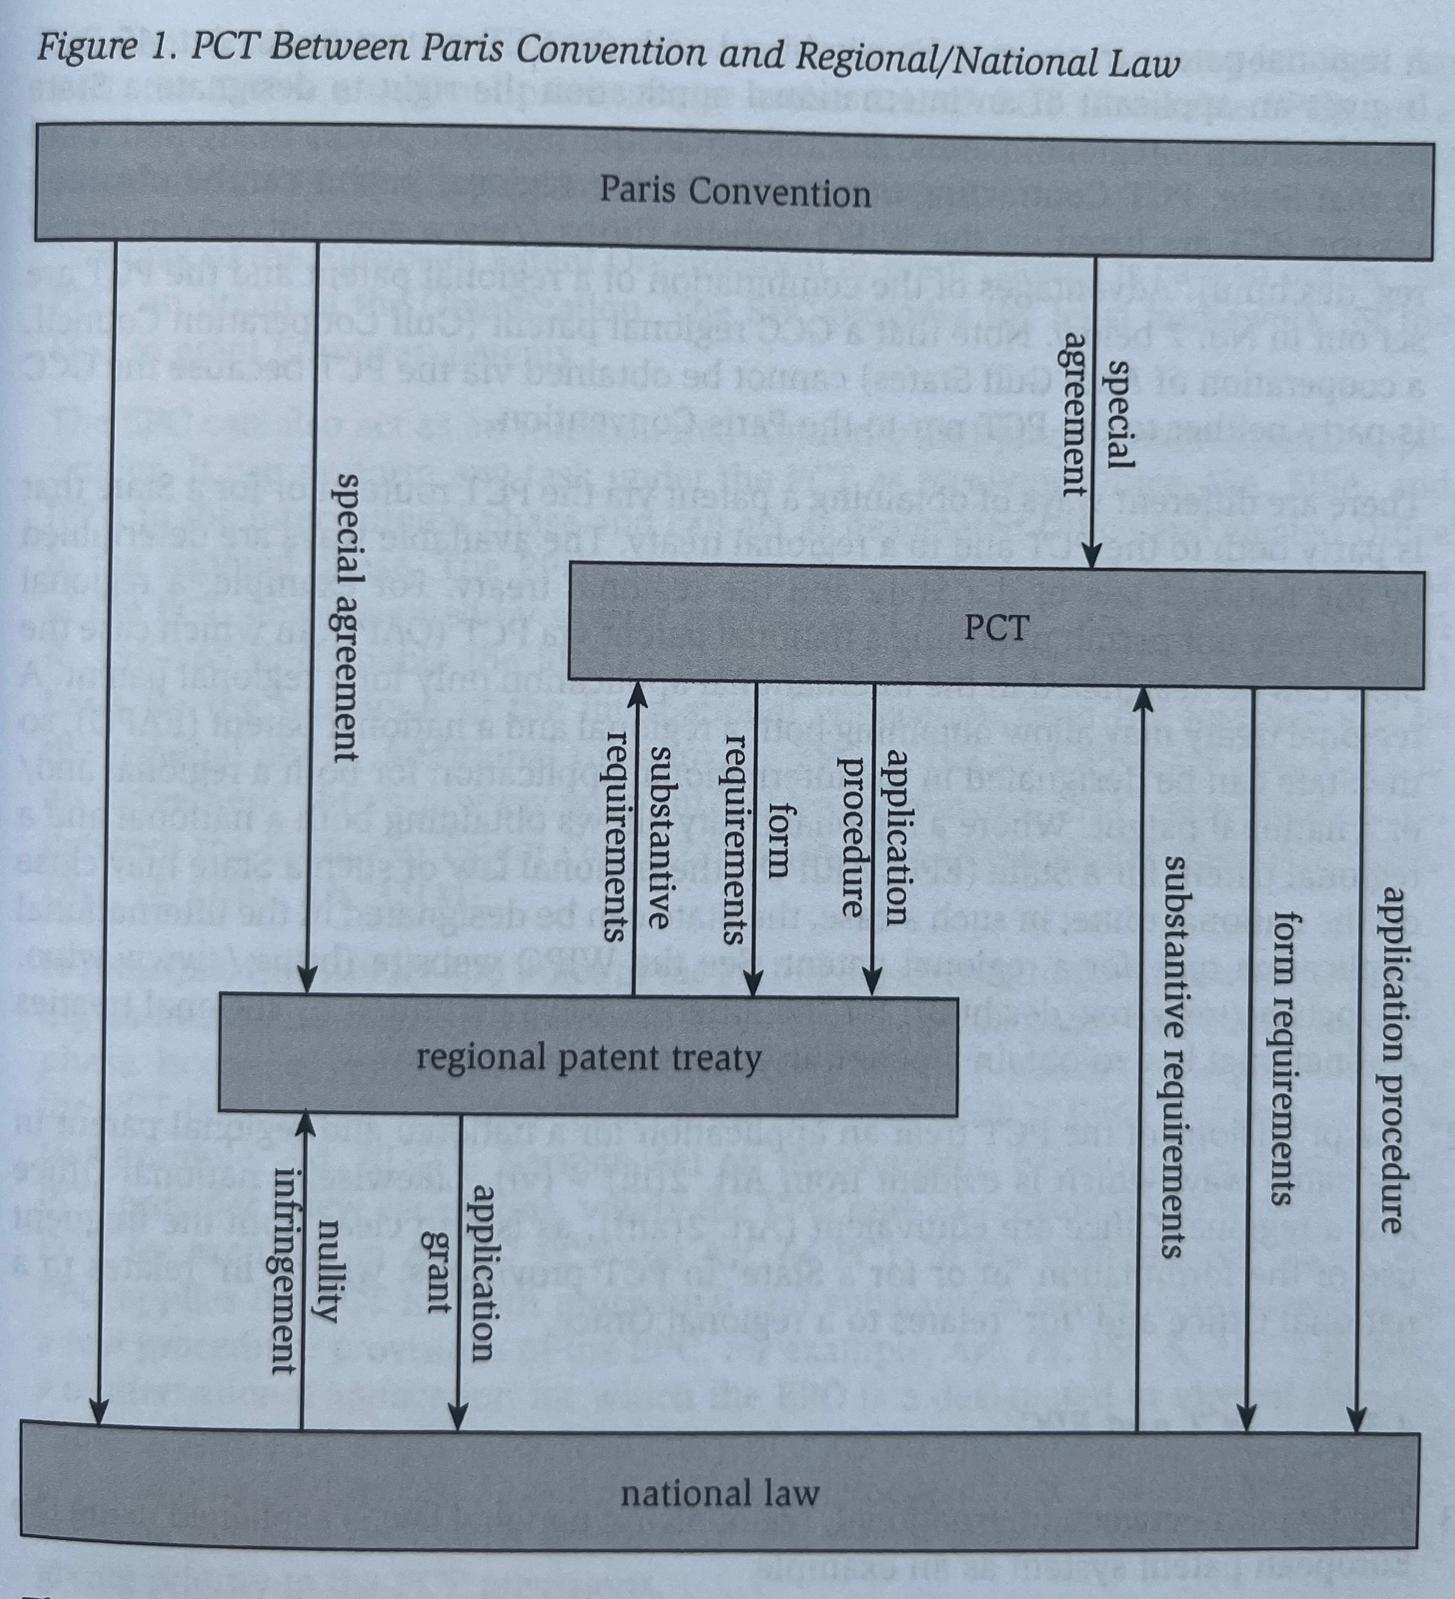
\includegraphics[width=0.6\textwidth]{images/Fig_1.jpg} % Pfad und Dateiname anpassen
  \caption{--- \textbf{\textsc{PCT Hierarchy}}}
\end{figure}

\p Agreement between countries for mutual recognition of IP rights. Nationals of Signatory Countries enjoy the same rights in other States as nationals of those other States. \n

\p It secured \textbf{the right of priority} of a first filing in one State for subsequent applications in other States. \n

\p A \textbf{priority right} is a time-limited right triggered by the \textbf{first filing} of an application for a patent, industrial design, or trademark. It allows the applicant to file a \textbf{subsequent application} in another country that is effectively treated as if filed on the date of the first application, known as the \textbf{priority date}. To use this right, the applicant (\textbf{or their successor in title}) must \textbf{claim priority} in the subsequent application. \n

\p The priority period is \textbf{12 months} for patents and utility models (the \textbf{priority year}) and \textbf{6 months} for industrial designs and trademarks. In the original Paris Convention it was 6 months and 3 months, respectively. \n

\p For patents, this right is crucial because \textbf{novelty} and \textbf{inventive step} are assessed against prior art that was made public \textbf{before the priority date}, not the actual (later) filing date of the subsequent application. \n

\nt{Rationale}{\textbf{according to the EPO: \textit{``(...) basic purpose [of the right of priority] is to safeguard, for a limited period, the interests of a patent applicant in his endeavour to obtain international protection for his invention, thereby alleviating the negative consequences of the principle of territoriality in patent law.''}}} 
\vspace{5mm}

\p \textbf{\s Art. 19} of the Paris Convention allows for special agreements between Signatory Countries. The Paris Convention \underline{takes precedence} over laws of the Countries and over such special agreements. \n

\p EPC is a ``regional patent treaty'' in the sense of \textbf{Art. 19} of the Paris Convention, e.g., under \textbf{Art. 45 PCT}, a PCT applicant can obtain an \underline{\underline{EP patent}} by filing an initial international application. \n

\nt{Definition}{\textbf{\[
    \begin{dcases}
        \mathrm{Patent \ \underline{in} \ a \ state} & = \ \ \mathrm{\underline{national}}\\
        \mathrm{Patent \ \underline{for} \ a \ state} & = \ \ \mathrm{\underline{regional}} \\
    \end{dcases}
\]}} 
\vspace{5mm}

\p Under \textbf{Art. 45 PCT}, a PCT Applicant can obtain a European patent by filing a PCTa. \n

\p In case of conflict between PCT and EPC/national provisions, the PCT takes precedence. \n

\p A ``Euro--PCT'' application is a PCT application with EPO as dO or eO. \n

\p The PCT timeline for a PCTa claiming priority from a national application: 

\newpage
\begin{figure}[H] % h=here, t=top, b=bottom, p=page: Platzierungs-Optionen
  \centering
  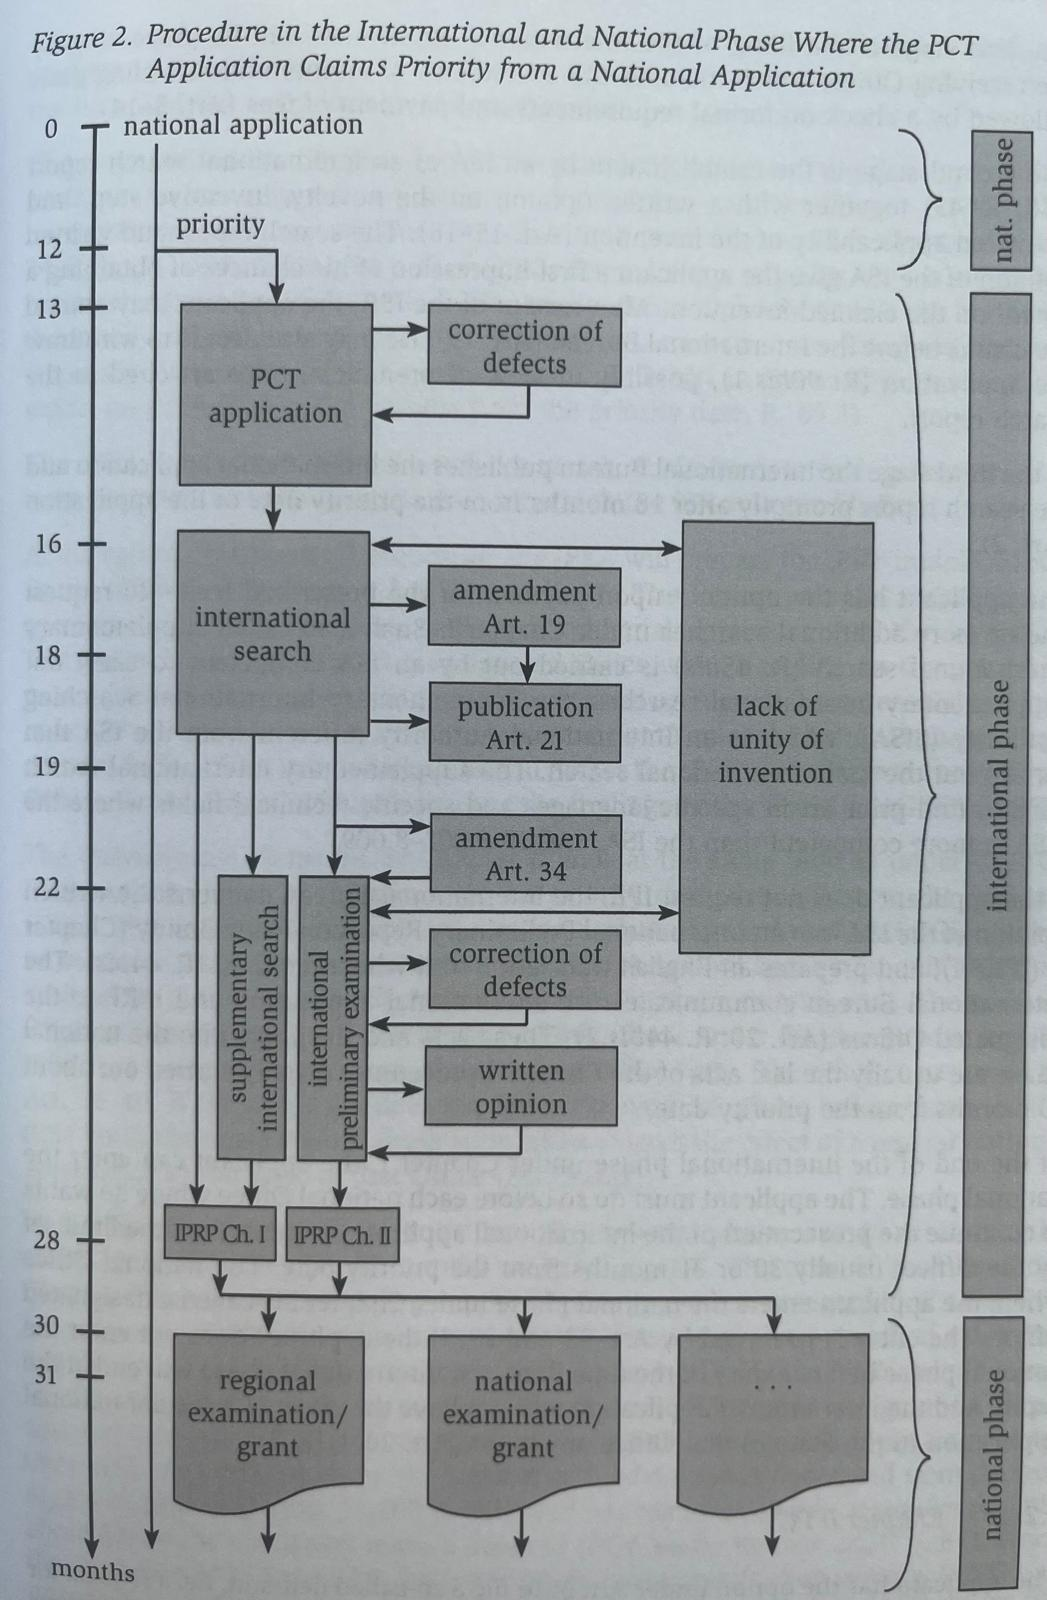
\includegraphics[width=0.85\textwidth]{images/Fig_2.jpg} % Pfad und Dateiname anpassen
  \caption{--- \textbf{\textsc{PCT Timeline}}}
\end{figure}




\p The international phase includes: international search, publication and (optionally) international preliminary examination. The international phase has a \underline{Chapter I} (\textbf{Art. 3--30}; \textbf{R. 3--52}) and a \underline{Chapter II} (\textbf{Art. 31--42}; \textbf{R. 53--78}). These correspond to search + pub and IPE. \n

\p Each nO has a time limit for entering national phase (usually 30 or 31 months from the priority date). A PCTa can be simultaneously in the international phase and in the national phase for some jurisdictions. \n

\nt{Chapter I}{\textbf{Stage 1}: filing, accordance of date, fees, formal requirements. \newline
\textbf{Stage 2}: ISR with written opinion on Novelty, IS and industrial applicability. \newline
\textbf{Stage 3}: publication of PCTa + ISR @18 months after priority date. } 
\vspace{5mm}


\nt{Chapter II}{\textbf{Stage 1}: filing a \underline{\textbf{demand}}, i.e., a request for an IPE --- typically @22 months after priority date.\newline
\textbf{Stage 2}: can amend claims and discuss Novelty, IS with Examiner. \newline
\textbf{Stage 3}: receipt of the \underline{IPRP II} typically @28 months from priority date. } 
\vspace{5mm}

\p Applicant can pay for a Supplementary ISR carried out by a SISA (can be different to ISA of Chapter I, e.g., in order to find prior art in a specific language.) \n

\p If no IPE demanded, written opinion from ISR is converted into the International Preliminary Report on Patentability I (\underline{IPRP I}) with an English translation thereof + documents are communicated to the dO. Usually happens @30 months after priority date.\n

\p IPRP is not binding on the dO but is made available to the dO. dO then becomes the eO.\n

\p Only about 3\% of applications ever enter Chapter II. \n


\p \textsc{LU} is a notable exception for entering national phase -- 20 months. \n

\p PCT advantages over direct national application include: 

\begin{itemize}
 \item cost reduction,
 \item 30-month delay to check market developments, own product developments, etc.,
 \item patentability opinion to inform later actions,
 \item delay of formalities/payments right away.
\end{itemize}

\p If no priority claim, then \textbf{the priority date is the PCTa filing date}. \n

\p ``Agent'' is ``professional representative'' in EPC terminology. \n

\p Terminology for document copies:

\begin{itemize}
\centering
 \item \textbf{Home copy} --- stays with rO.
 \item \textbf{Record copy} --- sent to IB.
 \item \textbf{Search copy} --- sent to ISA.
\end{itemize}

\p Record copy is the \textbf{true} copy. \n

\p It is possible that scope of PCTa only includes \textit{certain territories} of a CS, e.g., a Euro--PCT for Denmark does not include the Faroe Islands. \n

\p States can join to form a single legal territory for patent law, e.g., Switzerland and Liechtenstein. \n

\newpage

\chapter{The International Application (\textsc{PCTa})}

\section{Basics}

\p Elements that a PCTa must contain:

\begin{itemize}
 \item a request (\textbf{Art. 4)},
 \item a description (\textbf{Art. 5)},
 \item one or more claims (\textbf{Art. 6)},
 \item where required, one or more drawings (\textbf{Art. 7)},
 \item an abstract (\textbf{Art. 8)}.
\end{itemize}

\p To accord a \textbf{filing date}, you need:

\begin{itemize}
 \item an indication that it is inteded as a PCTa, including a designation of a Contracting State and name of Applicant,
 \item a description,
 \item at least one claim.
\end{itemize}

\p The Abstract may be submitted later though. \n

\p On filing, the description, claims and drawings may be replaced by \underline{reference to a priority application,} from which the rO will copy them [\textbf{R. 4.18} \& \textbf{R. 20.6}].

\section{Art. 3(4)(i) \& Rule 12 --- Languages and Translations}

\subsection{Languages accepted by the rO}

\p A PCTa must be filed in a language prescribed by the rO. \textbf{Every} rO accepts at least one language, which is \textbf{both} a language accepted by the competent ISA \underline{and} a language of publication. Languages of publication are listed under \textbf{R. 48.3(a)}. If using the language of publication, no translation need be filed.  \n

\p To get a filing date, claims and description must be in a language accepted by that rO. For cases of mixed languages of claims/description, an invitation to correct this will be issued under [\textbf{R. 26.3\textit{ter}(a)}]. \n

\p Languages of the request and the description/claims may be different though, e.g., an English request and Dutch claims/description. \n

\p The rO may require a translation for the purposes of search or publication, e.g., \textsc{RO/EP} requires \textbf{FR/EN/DE} translation. \n

\p All rOs of EPC CSs have specified the EPO as their competent ISA. Search in Dutch is possible at the EPO if the application was filed in Dutch for historical reasons. \n

\p The language of the rO need not be the official language of that CS. See also national security considerations under \textbf{Art. 27.8}, which may become relevant in such a case. \n

\p If a nO as rO does not accept the application language, it will transmit the PCTa to the IB to act as the rO under [\textbf{R. 19.4}]. IB accepts \textbf{any language}. In that case, new fees will need to be paid to the IB, the fees already paid to the nO will be refunded --- \textbf{except the transmittal fee} --- and the Applicant has to send the priority document to the IB. \n

\subsection{Translations}

\p The Applicant must provide a translation if:

\begin{enumerate}
 \item the language of filing is not accepted by the ISA (or SISA);
 \item the language of the ISA is not a publication language.
\end{enumerate}

\p The translation must be provided within \textbf{1 month of filing at the rO} -- otherwise a late furnishing fee is also due (equal to \textbf{25 \% of the international filing fee}). \n

\p The translation must be in the language of the ISA, language of publication \underline{and} language of the rO. Sequence listing free text needs to be translated as well. \n

\p If no translation is provided, the PCTa will be declared by the rO to have been withdrawn . \n

\p The rO will invite a translation witin 1 month of filing, if not received at filing. The late submission deadline is \textbf{2 months after filing} or \textbf{1 month after the invitation} -- whichever expires \textbf{later}. \n

\p Nonetheless, a translation and payment received before 15 months after priority date will be considered as received in time. Furthermore, a translation and payment received \textbf{before the rO makes the declaration} is also considered as received on time. \n

\p Under [\textbf{R. 12.4}] --- where a PCTa has been filed in a language accepted by the ISA, which is not a language of publication:

\begin{itemize}
 \item the Applicant must file a translation to a language of publication within \textbf{14 months} of the priority date;
 \item the rO will send an invitation for the late translation within \textbf{16 months} of the priority date;
 \item if the translation and late payment fee are received within \textbf{17 months} of the priority date, it is considered on time; and
 \item if the translation and late payment fee are received before the rO \textbf{declares withdrawal}, it is still considered on time.
\end{itemize}

\p PCT has a provision for retroactive scope limitation due to an incorrect translation under [\textbf{Art. 46}].

\section{Fees}

\p On filing of a PCTa, three fees (in Swiss francs) become due at the rO:

\begin{enumerate}
 \item transmittal fee;
 \item international filing fee (including sheet fee if $>$ 30 pages;
 \item international search fee.
\end{enumerate}

\p There are no claims fees. They may be due for some offices in the national phase. \n

\p PCT has no provisions for methods of payment or according a date of payment. Each rO will have its own rules on that. \n

\p The \textbf{transmittal fee} [\textbf{R. 14}] --- includes checking the PCTa, transmitting a record copy to the IB and the search copy to the ISA. The time limit for receipt is \textbf{1 month from the date of receipt of the application by the rO} (not from the filing date). The filing date might be shifted due to missing elements, etc., so the fees deadlines are not dependent on the filing date. This deadline is also shifted if the rO sends the PCTa to the IB when the rO is not the Competent Authority. \n

\p The \textbf{international filing fee} [\textbf{R. 15}] --- includes publication, translation/s and communication to ISA/SISA/IPEA. Must be paid before formalities check of \textbf{Art. 14(1)(a)} and any resulting corrections. The 30 pages limit before any extra fees is calculated on the basis of documents as filed. Within \textbf{1 month of date of receipt of the PCTa} again (not the filing date).




\newpage

\chapter{Fillun Homework Questions}

\section{September 22, 2025}

\begin{enumerate}[label=\textbf{Question \arabic*}]

    \item % Question 1
    Two applicants wish to appoint an agent to file their international application.
    \begin{enumerate}[label=(\alph*)]
        \item Who can be appointed to act as an agent?
        \item How must the agent be appointed?
        \item Do all receiving Offices require the filing of a separate power of attorney?
        \item Does the EPO require the filing of a separate power of attorney?
    \end{enumerate}
    
    \vspace{1em} % Adds a little vertical space
    The applicants always work via the same patent attorney office for which a general power of attorney has been prepared.
    
    \begin{enumerate}[label=(\alph*), resume]
        \item Is it necessary to attach a copy of the general power of attorney to the Request [PCT/RO/101]?
        \item Does the EPO require filing a copy of the general power of attorney?
    \end{enumerate}

    \item % Question 2
    An international application is filed at the Japanese National Office. The applicant first mentioned in the Request [PCT/RO/101] is a Taiwanese national resident in Taiwan. The second applicant is a Korean national resident in Korea and the third applicant is a Japanese national resident in Japan. The three applicants have not appointed a common agent or a common representative.
    \begin{enumerate}[label=(\alph*)]
        \item Who will be considered to be the common representative of the applicants?
        \item Would your answer to question (a) have been different if the international application had been filed at the International Bureau?
        \item Which acts may not be performed by the representative in question (a)?
        \item Which acts may not be performed by an agent appointed by the representative in question (a)?
    \end{enumerate}

    \item % Question 3
    Today, 16 March 2020, the applicant discovers an obvious mistake in the description of his international application filed on Friday 9 March 2018 as a first filing.
    \begin{enumerate}[label=(\alph*)]
        \item Can this obvious mistake be corrected? If so, what are the conditions?
        \item Who is competent to rectify the obvious mistake? What if the mistake is only detected after a demand for international preliminary examination has been made?
        \item What parts of the international application are taken into account upon correcting the mistake?
        \item When at the latest can a request for rectification be filed?
        \item Would your answer have been different if the applicant had discovered an obvious mistake in the abstract of his international application?
    \end{enumerate}

    \item % Question 4
    Is it possible to file third party observations in relation to an international application during the international phase? If so, where and how can these be filed?

    \item % Question 5
    A Danish applicant filed an international application PCT-DK as a first filing on 25 May 2025 with the EPO as receiving Office. Due to cash-flow problems, no fees were paid upon filing. On 30 June 2025, the EPO issues an invitation to pay the missing fees together with a late-payment surcharge.

    \vspace{1em}
    Indicate True/False:
    \begin{enumerate}[label=(\alph*)]
        \item If the applicant has, in fact, paid the fees due at filing on 27 June 2025, the payment will be considered in time.
        \item The time limit to pay the missing fees together with late-payment surcharge expires on 1 September 2025.
        \item If the applicant pays the missing fees + surcharge one day after the time limit to do so has expired, this is too late and the EPO is obliged to declare under Art. 14(3) that PCT-DK is considered withdrawn.
    \end{enumerate}

    \item % Question 6
    What happens if the applicant is a resident or national of one of the PCT Contracting States but files the international application with a "non-competent" receiving Office? What are the consequences for according the international filing date for such an application? Must an additional fee be paid?

\end{enumerate}

\begin{center}

\p \p \p
 
\end{center}

\begin{enumerate}[label=\textbf{Answer \arabic*}]

    \item % Question 1
    Two applicants wish to appoint an agent to file their international application.
    \begin{enumerate}[label=(\alph*)]
        \item Under \textbf{R. 90}: a person having the right to practice before the national Office with which the PCTa is filed \underline{or} having the right to practice before the IB as rO. The latter is governed by \textbf{Rule 83}, i.e., the agent must have a right to practice before the nO of the Contracting State of which the Applicant is a resident or national.
        \item Applicant enters and signs the name \textbf{and} address of the agent in the request \underline{or} the demand \underline{or} in a separate power of attorney (applicable to a \textbf{specific} PCTa) \underline{or} by a general power of attorney (applicable to \textbf{any} PCTa).
        \item No.
        \item No.

        \item Yes. It says so on the \textsc{[PCT/RO/101]} form.
        \item No. Waiver under \textbf{Rule 90.5(c)}. Two exceptions relating to suspicions as to the nature of the person performing acts apply.
    \end{enumerate}

    \item % Question 2
    An international application is filed at the Japanese National Office. The applicant first mentioned in the Request [PCT/RO/101] is a Taiwanese national resident in Taiwan. The second applicant is a Korean national resident in Korea and the third applicant is a Japanese national resident in Japan. The three applicants have not appointed a common agent or a common representative.
    \begin{enumerate}[label=(\alph*)]
        \item According to \textbf{Rule 90}, the first Applicant named in the Request entitled to file a PCTa with an rO will become the common representative. In this case, this should be the Korean national.
        \item No?
        \item The common representative may not sign any notice of withdrawal [under \textbf{R. 90\textit{bis}}], i.e.: withdrawal of application, designation, priority claim, supplementary search request, demand or election. Also, \textbf{not sure}, but it seems like he cannot perform an act in relation to only one Applicant or a subset of Applicants when there are multiple Applicants. 
        \item The common agent may not file a PCTa without signature of the Applicant/s [\textbf{R. 4.15}] and cannot make declarations as to entitlement on behalf of the Applicant/s [\textbf{R. 4.17}].
    \end{enumerate}

    \item % Question 3
    Today, 16 March 2020, the applicant discovers an obvious mistake in the description of his international application filed on Friday 9 March 2018 as a first filing.
    \begin{enumerate}[label=(\alph*)]
        \item Yes --- under \textbf{Rule 91.2}, there is a 26 month-deadline for correction of obvious mistakes. In this case, we have 24 months + 7 days.
        \item The Applicant (or his agent) are competent. After demand, the IPEA is the Competent Authority to be addressed. Notably, the dO/eO need not take rectification into account if processing/examination started prior to the notification [\textbf{R. 91.3(e)}] and the dO/eO may disregard an authorized notification if it finds it would not have authorized it itself had it been the Competent Authority [\textbf{R. 91.1(f)}].
        \item For mistakes in the claims, description or drawings (or corrections thereof), only the claims, description and drawings (and corrections thereof) will be taken into account [\textbf{R. 91.1(d)}]. 
        For mistakes in the Request (or corrections thereof), the contents of the whole PCTa including priority documents, corrections, etc., will be taken into account [\textbf{R. 91.1(e)}].
        \item 26 months after the priority date.
        \item Yes. Abstract mistakes may not be corrected under \textbf{Rule 91.1(g)}. They may be corrected under [\textbf{R. 38.3}] within \textbf{1 month} after the date of mailing of ISR by submission of corrections to the ISA.
    \end{enumerate}

    \item % Question 4
    Is it possible to file third party observations in relation to an international application during the international phase? If so, where and how can these be filed?


      Third party observations may be submitted at any time \textbf{after the date of publication} of the international application \underline{and} \textbf{before the expiration of 28 months from the priority date}, provided that the application is not withdrawn or considered withdrawn.
      
                They can be submitted through ePCT at no cost (you need a WIPO account). Each observation must                                                                                          include at least one citation that refers to a document published before the international                                         filing date, or a patent document having a priority date before the international filing date, together with a brief explanation of how each document is considered to be relevant to                                                                                                                                                                                                                                                                                                                                                                                                                                          the questions of novelty and/or inventive step of the claimed invention. Observations                                                                                                                                                                                                                                                                                                                                                                                                                                           should preferably be accompanied by a copy of each cited document.      They should be submitted in a language of publication (copies of prior art may be in any language). A single party may only submit a single observation for any PCTa, with a cap of ten observations (generally existing) per PCTa. 
                
                
                
                
                
    \item % Question 5                         
    A Danish applicant filed an international application PCT-DK as a first filing on 25 May 2025 with the EPO as receiving Office. Due to cash-flow problems, no fees were paid upon filing. On 30 June 2025, the EPO issues an invitation to pay the missing fees together with a late-payment surcharge.
                                                                                          
                                                                                          
    Indicate True/False:
    \begin{enumerate}[label=(\alph*)]
        \item \textbf{True} --- any payment received by rO before invitation to pay fees is considered to have been received before the time limit.
        \item \textbf{False} --- \textit{1 month} from the date of the invitation is the time limit. So it should be 30 July 2025.
        \item \textbf{False} --- any payment received before this declaration by the rO shall be considered to have been received before the expiration of the time limit. 
    \end{enumerate}

    \item % Question 6
    What happens if the applicant is a resident or national of one of the PCT Contracting States but files the international application with a "non-competent" receiving Office? What are the consequences for according the international filing date for such an application? Must an additional fee be paid?
    
    The PCTa will be considered to have been received by the Office with which it was filed on behalf of the IB as rO. The PCTa will be date-stamped by the nO (or regional Office) concerned and promptly submitted to the IB (unless for national security reasons).
    
    The filing date will be the date of receipt by the nO, but for calculating time limits for fee payments, the date on which the IB received the application will be used.
    
    That transmittal from nO to IB may be subjected to the payment of a fee equal to the transmittal fee, with other fees being refunded and then pending for payment again at the IB. 

\end{enumerate}

\section{September 29, 2025}

\begin{enumerate}[label=\textbf{Question \arabic*}]

    \item % Question 1
   An Austrian applicant A files an international application in German with the EPO. Before publication of the application, A sells this international application to US-company B, based in San Francisco, USA.
You are a European patent attorney representing company A and, after the purchase, company B in respect of this application.


For each of the statements below, indicate whether the statement is true or false:

    \begin{enumerate}[label=(\alph*)]
        \item  The change of applicant can be recorded by the IB during the international phase on request of the applicant (provided that the request is filed within the applicable time limit). 
\item A request to record the change of applicant can be filed with the EPO.
\item The change of applicant can be recorded by the IB during the national phase after the expiry of 30 months of priority date, with effect to all designated offices (provided that the request is filed within the applicable time limit).
\item The change of applicant can no longer be recorded during the international phase once international publication has taken place. 
\item The change of applicant can be recorded by the IB after the expiry of 30 months from the priority date until expiry of 31 months from the priority date, but such recordal only has effect with respect to the designated offices where the 31
month-period applies for national/regional entry.

   \end{enumerate}
    
    \item % Question 2
An applicant resident in Spain filed an international application in Spanish at the Spanish national Office indicating the EPO as International Searching Authority. Within one month the applicant furnishes pursuant to PCT Rule 12.3(a) a translation of the application into English.
    \begin{enumerate}[label=(\alph*)]
        \item   In which language will the international application be published?
\item  Which parts of the international application will (also) be published in English?
    \end{enumerate}

    \item % Question 3
A Dutch applicant filed a European patent application with the EPO on Friday 11 May 2018 comprising just a description and drawings, but no claims. On the same day, he filed the same documents with the IB together with a PCT Request Form. On Wednesday 23 May 2018, he filed a set of claims with the EPO and also with the IB, referring to his earlier submissions of 11 May 2018.


For each of the statements below, indicate whether the statement is true or false:

The filing date accorded to the European patent application is...


    \begin{enumerate}[label=(\alph*)]
        \item  … 11 May 2018.
\item … 23 May 2018.
    
\vspace{0.5cm}

The filing date accorded to the international patent application is ...
 
        \item  … 11 May 2018.
\item … 23 May 2018.
    \end{enumerate}

    \item % Question 4
An international application is jointly filed at the German national Office on 3 April 2017 by a British applicant and a German applicant claiming priority from an earlier German national application filed on 4 April 2016.


For each of the statements below, indicate whether the statement is true or false:

    \begin{enumerate}[label=(\alph*)]
        \item  All applicants must be indicated in the Request (PCT/RO/101).
\item The rO considers it sufficient if the British applicant signs the Request.
\item The receiving Office will invite the applicants to furnish any missing address, nationality and residence.
    
\vspace{0.5cm}

Later on the applicants wish to withdraw the priority claim.
 
        \item The priority claim may be withdrawn until 3 October 2019.
\item It is sufficient if the first-named applicant, being considered to be the common representative under R.90.2(b), signs the notice of withdrawal.
\item  If the applicants would have appointed a common representative, the common representative may sign the notice of withdrawal.


\vspace{0.5cm}

Later on the international application enters the regional phase before the EPO.


\item The EPO will ask for any missing indication of the applicants in the Request.


    \end{enumerate}


    \item % Question 5

An international application is filed on 28 July 2018 indicating a priority date of 27 January 2018. The applicant wishes to correct the priority date to 26 September 2017 and asks you until when may he can request the competent authority of a correction of the priority date. Today is 12 November 2018.

For each of the statements below, indicate whether the statement is true or false.

The last day to request the correction is...


    \begin{enumerate}[label=(\alph*)]
        \item  Wednesday 28 November 2018. 
\item Monday 28 January 2019.
\item Monday 27 May 2019.   
\vspace{0.5cm}

The request may be filed with…
 
        \item the receiving Office.
\item the International Bureau.



    \end{enumerate}

\item % Q6

    \begin{enumerate}[label=(\alph*)]
        \item  Can the applicant withdraw a priority claim made in the international application? If so, until when?
\item To whom must the request be addressed? Who must sign the withdrawal?
\item Is a fee due for the withdrawal of a priority claim? 

\item What are the consequences of a withdrawal of a priority claim?

     \end{enumerate}


\item % Q7

Today, Monday 27 November 2017, an applicant wants to file an international application at the EPO as receiving Office claiming the priority of an earlier national application filed on 24 September 2016.

    \begin{enumerate}[label=(\alph*)]
        \item  Is it still possible to file the international application and claim the priority?
\item  If so, how must the applicant proceed?
\item Do all rOs accept such requests?

\item Are dOs required to accept the claimed priority?
\item What about the EPO?

     \end{enumerate}
       \end{enumerate}

       \section{October 09, 2025}

\begin{enumerate}[label=\textbf{Question \arabic*}]

    \item % Question 1
    L3-06 - T/F question (Basic selection) \\
    An international application is filed by a Danish national at the Danish Patent and Trademark Office as receiving Office. \\
    For each of the statements below, indicate whether the statement is true or false.
    \begin{enumerate}[label=(\alph*)]
        \item The IA may be filed in…
        \begin{enumerate}[label={(\alph{enumi}.\arabic*)}]
            \item ... Danish
            \item ... English
            \item ... Swedish
        \end{enumerate}

        \item The applicant may select as ISA:
        \begin{enumerate}[label={(\alph{enumi}.\arabic*)}]
            \item ... the Danish national office.
            \item ... the EPO
            \item ... the Swedish national office.
            \item ... the Nordic Patent Institute.
        \end{enumerate}
        
        \item \textit{The application is filed in Danish.} \\
        For each of the statements below, indicate whether the statement is true or false
        
        \vspace{0.5em}
        The EPO as ISA…
        \begin{enumerate}[label={(\alph{enumi}.\arabic*)}]
            \item ... does not require a translation for the purposes of international search.
            \item ... requires a translation into any one of the 10 publication languages for the purposes of international search.
            \item ... requires a translation into English, French or German for the purposes of international search.
            \item[] \textit{The Nordic Patent Institute as ISA...}
            \item ... does not require a translation for the purposes of international search.
            \item ... requires a translation into any one of the 10 publication languages for the purposes of international search.
            \item ... requires a translation into English, French or German for the purposes of international search.
        \end{enumerate}

        \item \textit{The applicant has filed the international application in Danish and has indicated the EPO as International Searching Authority. The applicant is in the progress of making a translation into English. The application was filed by fax with the Danish Patent and Trademark Office on a day on which the Danish Patent and Trademark Office and the International Bureau were closed.} \\
        For each of the statements below, indicate whether the statement is true or false: \\
        The translation must be filed ...
        \begin{enumerate}[label={(\alph{enumi}.\arabic*)}]
            \item ... within one month from the date of receipt by the Danish Patent and Trademark Office to avoid any late furnishing fee(s).
            \item ... within one month from the date of receipt by the EPO to avoid any late furnishing fee(s).
            \item ... when the 1m period was missed, the translation may still be provided as long as a late furnishing fee is paid.
            \item ... when the rO issues an invitation to supply a missing translation, the ultimate time limit to respond is always one month from the date of the invitation.
        \end{enumerate}
        
        \item \textit{The applicant has timely filed the translation into English to the Danish Patent and Trademark Office.} \\
        The international publication of the international application will take place in…
        \begin{enumerate}[label={(\alph{enumi}.\arabic*)}]
            \item ... Danish.
            \item ... English.
            \item ... in Danish with the title and the abstract also in English.
        \end{enumerate}
    \end{enumerate}

    \item % Question 2
    L3-08 - T/F question (Basic selection) \\
    A PCT application was filed with the EPO. As the International Searching Authority, the EPO considered that the application was not unitary. The invention first mentioned in the claims was searched and an invitation to pay two additional international search fees was sent to the applicant last week, 8 March 2023. The third invention, which has not yet been searched, is the only invention that the applicant would like to pursue in the European phase before the EPO. \\
    Today is 17 March 2023.
    \begin{enumerate}[label=(\alph*)]
        \item For each of the statements below, indicate whether the statement is true or false:
        \begin{enumerate}[label={(\alph{enumi}.\arabic*)}]
            \item In the international PCT phase, the applicant can file a protest with the EPO and request that a full search is made. The protest is free of charge, but it has to be supported by arguments.
            \item The applicant can timely pay one additional fee for the third invention to be searched in the international PCT phase. In the European phase, the applicant can limit the application to the third invention.
            \item The applicant can ignore the invitation. In the European phase, the applicant can file a divisional application directed to the third invention.
            \item The applicant can ignore the invitation. In the European phase, the applicant will again receive an invitation to pay additional search fees.
        \end{enumerate}
        
        \item (from L3-14)
        \begin{enumerate}[label={(\alph{enumi}.\arabic*)}]
            \item What is the purpose of the requirement of "unity of invention"?
            \item What is the time limit to pay the additional search fee in the international phase?
            \item To whom must the additional search fee be paid?
            \item When must the applicant pay a "protest fee"? What time limit applies?
        \end{enumerate}
    \end{enumerate}

    \item % Question 3
    L3-16 
    \begin{enumerate}[label=(\alph*)]
        \item When must the international search report be established?
        \item What are the contents of the international search report?
        \item What can the applicant do after receiving the international search report, apart from filing a demand for international preliminary examination?
        \item What time limits apply? Where must the applicant file the amendments?
        \item In what form must the applicant file the amendments and any accompanying letter or statement? In which language?
        \item When are amendments to the claims under PCT Article 19 not allowed?
    \end{enumerate}

    \item % Question 4
    L3-20 (Basic selection) \\
    An applicant has filed an international application on 9 May 2023 as a first filing at the EPO as receiving Office, in English. The EPO acted as International Searching Authority and the international search report was transmitted to the applicant in December 2023; the written opinion (WO-ISA) suggests that the invention is patentable. \\
    The applicant being afraid that there is prior art which was not discovered by the EPO as ISA, considers filing a request for supplementary international search to be carried out by the Intellectual Property Office of Singapore.
    \begin{enumerate}[label=(\alph*)]
        \item Until when can the applicant file a request for supplementary international search [PCT/IB/375]? Where should the request be filed? In which language should the request be filed?
        \item What fees must be paid in respect of the request for supplementary international search? By when must the fees be paid? What is the amount of the fees?
        \item When will the supplementary international search start?
        \item By when must the supplementary international search report be established? Will a written opinion be issued together with the supplementary international search report?
        \item Will the supplementary international search report cite any document which was already cited in the international search report established by the EPO?
        \item Will the supplementary international search report be published? If so, in what form?
    \end{enumerate}

    \item % Question 5
    L3-27 \\
    A US applicant wants to request a demand for international preliminary examination at the USPTO for an international application filed on 29 December 2016 without any claiming priority. The ISR and WO-ISA, established by the USPTO as ISA, were transmitted to the applicant on 26 June 2018. \\
    However, due to a severe hurricane, the USPTO was closed on 29 and 30 October 2018, and the applicant was not able to submit the demand on 29 October 2018. \\
    Can the demand still be validly filed if today is 31 October 2018?

    \item % Question 6
    In which cases can the EPO act as IPEA? \\
    (multiple choice)
    \begin{enumerate}[label=(\alph*)]
        \item Spanish office was the ISA
        \item Nordic Patent Institute was the ISA
        \item USPTO was the ISA
        \item EPO was the ISA
    \end{enumerate}

    \item % Question 7
    What documents must an applicant file when filing Article 19 amendments? \\
    (single choice)
    \begin{enumerate}[label=(\alph*)]
        \item Only the amended claims \& a letter indicating the differences plus the basis for the amendments
        \item A complete set of claims in replacement of the claims originally filed \& a letter indicating the differences plus the basis for the amendments 
        \item Only the amended claims \& a letter indicating the differences plus the basis for the amendments \& statement by the applicant explaining the amendment and indicating any impact it might have on the description and the drawings
        \item A complete set of claims in replacement of the claims originally filed \& a letter indicating the differences plus the basis for the amendments \& statement by the applicant explaining the amendment and indicating any impact it might have on the description and the drawings
    \end{enumerate}

    \section{October 20, 2025}

\begin{enumerate}[label=\textbf{Question \arabic*}]

    \item % Question 1
    L4-06 (Basic selection) \\
    A US applicant, resident in the US, files his international application at the USPTO. Subsequently he wishes to pursue his application before the EPO as designated office.
    \begin{enumerate}[label=(\alph*)]
        \item Can the US applicant initiate the national entry procedure himself?
        \item What happens if a representative is not appointed once the processing has started by the EPO?
        \item What are the minimum acts to enter the regional phase before the EPO if surcharges are to be avoided?
    \end{enumerate}

    \item % Question 2
    L4-12 - T/F question (Basic selection) \\
    An international application was published in Korean together with the international search report established by the Korean patent office as ISA. The international application does not claim priority. The applicant wants to enter the European regional phase today, the last day of the 31-month period without any penalty fees. \\
    Which fees need to be paid within what time limit to avoid any penalty fees?

    \vspace{1em}
    For each of the statements below, indicate whether the statement is true or false.
    
    \vspace{0.5em}
    The examination fee….
    \begin{enumerate}[label=(\alph*)]
        \item ... needs to be paid upon entry today.
        \item ... may be paid, without any additional fee, until 6 months from the publication of the translation of the international application under Art.153(4) EPC, first sentence, as the publication of the translation comprises the translation of the international search report.
        \item ... may be paid, without any additional fee, until 6 months from the mention of the supplementary European search report in the European patent Bulletin.
        \item ... will be refunded if the applicant already paid the examination fee on entry and withdraws the application shortly after receipt of the supplementary European search report.
    \end{enumerate}

    \item % Question 3
    L4-22 \\
    How many claims fees must the applicant pay or does he get refunded, and when, in the following cases:
    
    \vspace{1em}
    \textbf{Case 1:} A Euro-PCT application X contains 27 claims on expiry of the 31-month period. The applicant pays five claims fees within the 31 month period. No amendments are filed after expiry of the 31-month period and before expiry of the six-month period under Rule 161.
    
    \vspace{1em}
    \textbf{Case 2:} A Euro-PCT application Y contains 27 claims on expiry of the 31-month period. The applicant pays five claims fees within the 31-month period. After expiry of the 31-month period and before expiry of the six-month period under Rule 161, the applicant files an amended set of 32 claims.

    \item % Question 4
    L4-23 (Basic selection) \\
    An international application is filed on 7 September 2015 without claiming priority. The applicant wants to enter the regional phase before the EPO as designated Office. Today is 26 February 2018. \\
    What is the last day on which the renewal fee in respect of the third year can be paid to the EPO…
    \begin{enumerate}[label=(\alph*)]
        \item ... without additional fee?
        \item ... with additional fee?
    \end{enumerate}

    \vspace{1em}
    L4-24 \\
    An international application is filed on 9 June 2016 claiming priority of a national application filed on 7 September 2015. The applicant wants to enter the regional phase before the EPO as designated Office. Today is 26 February 2018. \\
    What is the last day on which the renewal fee in respect of the third year can be paid to the EPO…
    \begin{enumerate}[label=(\alph*), resume]
        \item … without additional fee?
        \item … with additional fee?
    \end{enumerate}

    \item % Question 5
    L4-30 (Basic selection) \\
    A Swedish applicant has filed an international application indicating the Swedish Patent and Registration Office as International Searching Authority. The application is filed in English. During the international search, the ISA is of the opinion that the international application contains 3 inventions, A, B and C, and that with respect to the second and third invention an additional fee has to be paid for each of them if the International Search Report is to cover these inventions. An additional fee is only paid for the second invention B. No demand was filed. The applicant wants to enter the regional phase before the EPO in May 2023, and let the EPO conduct searches on all three inventions A, B and C in the regional phase before deciding with which invention to continue into examination.
    
    \vspace{1em}
    Which amount of search fee(s) and/or further search fees must the applicant pay at or shortly after entry into the regional phase before the EPO (assuming the EPO shares the non-unity opinion)?

    \item % Question 6
    L4-41 (Basic selection) \\
    Today, 25 February 2019, your Japanese client asks you to enter the regional phase before the EPO for a PCT-application filed in Japanese with the Japanese Patent Office on 26 July 2017, validly claiming priority from a Japanese patent application P-JP dated 1 August 2016. The International Preliminary Examination was carried out by the Japanese Patent Office. Due to an overload of work in the translation department of your client, you are informed that you will receive the English translation of the PCT-application on 23 April 2019.
    
    \vspace{1em}
    How would you proceed in order to enter the regional phase, keeping costs for your client to a minimum?

    \item % Question 7
    L4-42 (Advanced selection) \\
    An applicant wanted to enter the EP phase with his international application and duly filed a translation into English, and paid the filing fee and search fee. Shortly after the 31m time limit, the applicant received a loss-of-rights communication, indicating that the application was deemed to be withdrawn due to non-payment of the designation and examination fee and not filing the request for examination. One week after having received the communication, the applicant got into the hospital and despite all due care, he missed the time limit to request further processing with respect to the missed periods. 
    
    \vspace{1em}
    How many re-establishment fees does the applicant need to pay? 

\end{enumerate}
 \section{October 27, 2025}


\begin{enumerate}[label=\textbf{Question \arabic*}]

    \item % Question 1
    B4-02 \quad T/F question (Basic selection) \\
    Today is late February 2025. A Dutchman living in Sweden wishes to file a European patent application at the EPO in Munich via a Polish friend, who is a European patent attorney.
    
    \begin{enumerate}[label=(\alph*)]
        \item For each of the statements below, indicate whether the statement is true or false.
        \begin{enumerate}[label={(\alph{enumi}.\arabic*)}]
            \item The Dutchman is entitled to file the European patent application in Dutch.
            \item The Dutchman is entitled to file the European patent application in Swedish.
            \item The Dutchman is entitled to file the European patent application in Polish.
            \item The Dutchman is entitled to file the European patent application in German.
        \end{enumerate}
        
        \item For each of the statements below, indicate whether the statement is true or false
        \begin{enumerate}[label={(\alph{enumi}.\arabic*)}]
            \item The Dutchman is entitled to a reduction of the filing fee under R.7a(1) when the European patent application is filed in Dutch, and a translation into English is filed at the same time.
            \item The Dutchman is entitled to a reduction of the filing fee under R.7a(1) when the European patent application is filed in Swedish, and a translation into English is filed at the same time.
            \item The Dutchman is entitled to a reduction of the filing fee under R.7a(1) when the European patent application is filed in Polish, and a translation into English is filed at the same time.
            \item The Dutchman is entitled to a reduction of the filing fee under R.7a(1) when the European patent application is filed in German, and a translation into English is filed at the same time.
            \item The reduction of the filing fee that the Dutchman is entitled to under R.7a(1) if the relevant requirements as to languages, translations and time limits are met is 20\% of the filing fee, including a 20\% reduction of any "page fees".
            \item The reduction of the filing fee that the Dutchman is entitled to under R.7a(1) if the relevant requirements as to languages, translations and time limits are met is 30\% of the filing fee, including a 30\% reduction of any "page fees".
            \item The reduction of the filing fee that the Dutchman is entitled to under R.7a(1) if the relevant requirements as to languages, translations and time limits are met is 50\% of the filing fee, including a 50\% reduction of any “page fees".
            \item The Dutchman is (also) entitled to a reduction of the filing fee under R.7a(3) when the European patent application is filed in any language, and, where applicable, a translation into an official EPO language is filed at the same time.
        \end{enumerate}
        
        \item For each of the statements below, indicate whether the statement is true or false.
        \begin{enumerate}[label={(\alph{enumi}.\arabic*)}]
            \item The Dutchman is entitled to a reduction of the filing fee under R.7a(1) when the European patent application is filed in Dutch, and a translation into French is filed at the same time.
            \item The Dutchman is entitled to a reduction of the filing fee under R.7a(1) when the European patent application is filed in Dutch, and a translation into German is filed at the same time.
            \item The Dutchman is entitled to a reduction of the filing fee under R.7a(1) when the European patent application is filed in Dutch, and a translation into English is filed a week later.
            \item The Dutchman is entitled to a reduction of the filing fee under R.7a(1) when the European patent application is filed in English, and a translation into Dutch is filed a week later.
        \end{enumerate}
        
        \item \textit{Upon filing the EP application in Dutch by the Polish friend, the friend also pays all necessary fees.} \\
        For each of the statements below, indicate whether the statement is true or false.
        \begin{enumerate}[label={(\alph{enumi}.\arabic*)}]
            \item The EP application is validly filed when the EP application is filed in Dutch, and a translation into English is filed at own motion, without an invitation from the EPO, one week later.
            \item The EP application is validly filed when the EP application is filed in Dutch, and a translation into English is filed six weeks of filing the application.
            \item The EP application is validly filed when the EP application is filed in Dutch, and a translation into English is filed three months after of filing the application.
            \item If no translation is filed within 1 month of filing the EP application in Dutch, the EPO will issue an invitation to file a translation into an official EPO language within a time limit of two months.
        \end{enumerate}
    \end{enumerate}

    \item % Question 2
    B4-07
    \begin{enumerate}[label=(\alph*)]
        \item Which documents filed after filing the European patent application may a Dutch person file in Dutch?
        \item Must a translation be filed? In what language? What period applies?
        \item What is the consequence if a required translation is not filed?
    \end{enumerate}

    \item % Question 3
    B4-08 \quad T/F question (Basic selection) \\
    A European patent EP1 has been granted in English.
    
    \begin{enumerate}[label=(\alph*)]
        \item Mr. Jansen, a Dutch national living in the Netherlands, wants to file an opposition against European patent EP1. \\
        For each of the statements below, indicate whether the statement is true or false.
        \begin{enumerate}[label={(\alph{enumi}.\arabic*)}]
            \item Mr. Jansen may file the notice of opposition in Dutch.
            \item Mr. Jansen may file the notice of opposition in English.
            \item Mr. Jansen may file the notice of opposition in German.
            \item Mr. Jansen may file the notice of opposition in Chinese.
            \item Mr. Jansen may file the notice of opposition in Korean.
        \end{enumerate}
        
        \item Mr. Xiao, a Chinese national living in the Netherlands, wants to file an opposition against European patent EP1. \\
        For each of the statements below, indicate whether the statement is true or false.
        \begin{enumerate}[label={(\alph{enumi}.\arabic*)}]
            \item Mr. Xiao may file the notice of opposition in Dutch.
            \item Mr. Xiao may file the notice of opposition in English.
            \item Mr. Xiao may file the notice of opposition in German.
            \item Mr. Xiao may file the notice of opposition in Chinese.
            \item Mr. Xiao may file the notice of opposition in Korean.
        \end{enumerate}
        
        \item Mrs. Lee, a Korean national living in Korea, wants to file an opposition against European patent EP1 via Mr. Koch, her European patent attorney based in Munich. \\
        For each of the statements below, indicate whether the statement is true or false.
        \begin{enumerate}[label={(\alph{enumi}.\arabic*)}]
            \item Mrs. Lee may file the notice of opposition in Dutch through Mr. Koch.
            \item Mrs. Lee may file the notice of opposition in English through Mr. Koch.
            \item Mrs. Lee may file the notice of opposition in German through Mr. Koch.
            \item Mrs. Lee may file the notice of opposition in Chinese through Mr. Koch.
            \item Mrs. Lee may file the notice of opposition in Korean through Mr. Koch.
        \end{enumerate}
    \end{enumerate}

    \item % Question 4
    B4-13 \quad T/F question (Advanced selection) \\
    A European patent application has been filed in Swedish by a Danish applicant living in Sweden. A translation of the patent application into English was duly filed. In reply to a communication from the Examining Division setting a period of 4 months to respond, the applicant files, on the last day of the period:
    \begin{itemize}
        \item a letter with his observations in Danish,
        \item in an Annex amendments to the claims in Swedish, and 
        \item in a further Annex as evidence a Japanese patent application in Japanese.
    \end{itemize}
    
    \begin{enumerate}[label=(\alph*)]
        \item For each of the statements below, indicate whether the statement with regard to the letter is true or false.
        \begin{enumerate}[label={(\alph{enumi}.\arabic*)}]
            \item The letter is filed in a non-admissible language, so the letter is deemed not filed.
            \item A translation of the letter has to be filed within 1 month of filing the letter. The translation has to be into English.
            \item A translation of the letter has to be filed within 1 month of filing the letter. The translation has to be into any one of English, French or German.
            \item If the applicant fails to file a translation within the required time limit, the letter is deemed not filed.
            \item If the applicant fails to file a translation of the letter nor of the claims within the required time limit, the application is deemed withdrawn.
        \end{enumerate}
        
        \item For each of the statements below, indicate whether the statement with regard to the Annex with amendments to the claims is true or false.
        \begin{enumerate}[label={(\alph{enumi}.\arabic*)}]
            \item The claims are filed in a non-admissible language, so the amended claims are deemed not filed.
            \item A translation of the amended claims has to be filed within 1 month of filing the amended claims. The translation has to be into English.
            \item A translation of the amended claims has to be filed within 1 month of filing the amended claims. The translation has to be into any one of English, French or German.
            \item If the applicant fails to file a translation within the required time limit, the amended claims are deemed not filed.
            \item If the applicant fails to file a translation of the claims nor of the letter within the required time limit, the application is deemed withdrawn.
        \end{enumerate}
        
        \item For each of the statements below, indicate whether the statement with regard to the Annex with the Japanese patent application is true or false.
        \begin{enumerate}[label={(\alph{enumi}.\arabic*)}]
            \item The Japanese patent application is filed in a non-admissible language, so the Japanese patent application is deemed not filed.
            \item A translation of the Japanese patent application has to be filed within 1 month of filing the letter. The translation has to be into English.
            \item A translation of the Japanese patent application has to be filed within 1 month of filing the letter. The translation has to be into any one of English, French or German.
            \item If the applicant fails to file a translation within the required time limit, the Japanese patent application is deemed not filed.
            \item If the applicant fails to file a translation within the required time limit, the application is deemed withdrawn.
        \end{enumerate}
    \end{enumerate}

    \item % Question 5
    B4-17 (Basic selection) \\
    An Italian applicant files two European patent applications, EP1, which claims the priority of Italian application IT1, and EP2, which claims the priority of Italian application IT2. 
    EP1 is filed in Italian and is identical to IT1. An English translation of EP1 is supplied to the EPO two weeks later.
    EP2 is filed in English. It is the translation of IT2. 
    During the examination procedure, the English texts of EP1 and EP2 are found to contain translation errors.
    
    \begin{enumerate}[label=(\alph*)]
        \item Would it be possible to correct these errors for EP1?
        \item Would it be possible to correct these errors for EP2?
    \end{enumerate}

    \item % Question 6
    B5-08 \quad T/F question (Basic selection) \\
    A Dutch national lives in the USA and wishes to file a European patent application.
    
    \begin{enumerate}[label=(\alph*)]
        \item For each of the statements below, indicate whether the statement is true or false.
        \begin{enumerate}[label={(\alph{enumi}.\arabic*)}]
            \item He does not need to appoint a professional representative for filing a European patent application in Dutch at the EPO, but he can do so.
            \item He does not need to appoint a professional representative for filing a European patent application in English at the EPO, but he can do so.
        \end{enumerate}
        
        \item For each of the statements below, indicate whether the statement is true or false.
        \begin{enumerate}[label={(\alph{enumi}.\arabic*)}]
            \item He does not need to appoint a professional representative for paying the filing fee and search fee to the EPO, but he can do so.
            \item He does not need to appoint a professional representative for paying the filing fee and search fee to the EPO if he pays the fees simultaneously with filing the application, but he shall appoint a professional representative when the fees are paid later.
            \item He is obliged to let a professional representative pay the filing fee and search fee to the EPO.
        \end{enumerate}
        
        \item \textit{The Dutch national living in the USA files a European patent application at the EPO in Dutch.} \\
        For each of the statements below, indicate whether the statement is true or false.
        \begin{enumerate}[label={(\alph{enumi}.\arabic*)}]
            \item He does not need to appoint a professional representative when he files a translation in English 3 weeks after the filing date, but he can do so.
            \item He does not need to appoint a professional representative when he files a translation in English simultaneously with filing the application in Dutch.
        \end{enumerate}
        
        \item \textit{The Dutch national files only a fully completed request form, but does not file a description nor a reference to a previously filed application, nor any claims.} \\
        For the statement below, indicate whether the statement is true or false.
        \begin{enumerate}[label={(\alph{enumi}.\arabic*)}]
            \item He does not need to appoint a professional representative when he files a description 5 days after having filed the request form.
        \end{enumerate}
        
        \item \textit{The Dutch national files only a fully completed request form as well as a description but no claims.} \\
        For the statement below, indicate whether the statement is true or false.
        \begin{enumerate}[label={(\alph{enumi}.\arabic*)}]
            \item He does not need to appoint a professional representative when he files a set of claims 5 days after having filed the request form.
        \end{enumerate}
    \end{enumerate}

    \item % Question 7
    B5-09 (Basic selection) \\
    Who is deemed to be the common representative for a European patent application with three applicants, where no common representative has been appointed, in the following situations?
    
    \begin{enumerate}[label=(\alph*)]
        \item All applicants are from a Contracting State and none has appointed a professional representative.
        \item All applicants are from a Contracting State and applicant 3 has appointed a professional representative.
        \item Applicant 1 and 3 are from a Contracting State; applicant 2 is a US company; no professional representative has been appointed.
        \item Applicant 1 and 3 are from a Contracting State; applicant 2 is a US company; applicant 1 has appointed a professional representative.
        \item Applicant 1 and 3 are from a Contracting State; applicant 2 is a US company; applicant 3 has appointed a professional representative.
    \end{enumerate}

\end{enumerate}
\end{enumerate}

\begin{center}

\p \p \p
 
\end{center}

\begin{enumerate}[label=\textbf{Answer \arabic*}]

    \item % Question 1
   An Austrian applicant A files an international application in German with the EPO. Before publication of the application, A sells this international application to US-company B, based in San Francisco, USA.
You are a European patent attorney representing company A and, after the purchase, company B in respect of this application.


For each of the statements below, indicate whether the statement is true or false:

    \begin{enumerate}[label=(\alph*)]
        \item  \textbf{\textsc{True}} --- [\textbf{R. 92\textit{bis}.1}] deals with recording of changes in certain indications
in the Request or the Demand. Data changes on Applicant/Common Representative/Common Agent will be recorded by the IB up until 30 months after priority date. 
\item  \textbf{\textsc{True}} --- it may be filed with the rO (in this case, the EPO), but it is strongly recommended to go directly to the IB especially if closer to the 30-month deadline. 
\item  \textbf{\textsc{False}} --- [\textbf{R. 92\textit{bis}.1(b)} \& \textsc{AG--IP 11.021}] make it clear that after the deadline, the change must be requested directly with the dO/eO. 
\item \textbf{\textsc{False}} --- if change is to be taken into account before international publication, it should reach the IB before deadline for technical preparations, i.e., 1 day before the 15$^{\mathrm{th}}$ day before scheduled publication (see also: [\textsc{AG--IP 9.014}]).
\item \textbf{\textsc{False}} --- [\textbf{R. 92\textit{bis}.1(b)} \& \textsc{AG--IP 11.021}] make it clear that after the deadline, the change must be requested directly with the dO/eO, regardless of exact limit for entry into national/regional phase. 
    \end{enumerate}



    \item % Question 2
An applicant resident in Spain filed an international application in Spanish at the Spanish national Office indicating the EPO as International Searching Authority. Within one month the applicant furnishes pursuant to PCT Rule 12.3(a) a translation of the application into English.
    \begin{enumerate}[label=(\alph*)]
        \item  Spanish --- because it is a language of publication and the PCTa was filed in the language of publication [\textbf{R. 48.3(a)}].
\item  The declaration under \textbf{Art. 17.2(a)} [\textit{i.e., non-patentability}], the title of invention, the abstract and any text matter pertaining to the figure accompanying the abstract shall be published in English by the IB [\textbf{R. 48.3(a)}].
    \end{enumerate}

   \item % Question 3
A Dutch applicant filed a European patent application with the EPO on Friday 11 May 2018 comprising just a description and drawings, but no claims. On the same day, he filed the same documents with the IB together with a PCT Request Form. On Wednesday 23 May 2018, he filed a set of claims with the EPO and also with the IB, referring to his earlier submissions of 11 May 2018.


For each of the statements below, indicate whether the statement is true or false:

The filing date accorded to the European patent application is...


    \begin{enumerate}[label=(\alph*)]
        \item  … 11 May 2018. –––   \textbf{\textsc{True}}. For EP you don't need a claim to accord a filing date. Assuming other formalities such as name of Applicant, indication a patent is sought, etc., have also been provided.
\item … 23 May 2018. 
    
\vspace{0.5cm}

The filing date accorded to the international patent application is ...
 
        \item  … 11 May 2018.
\item … 23 May 2018. –––   \textbf{\textsc{True}}. For PCT, you need a claim to accord a filing date. He filed the claim/s within the 2-month deadline of \textbf{Rule 20.3(b)(i)}, so he will get a filing date on the later date within this 2-month window.
    \end{enumerate}
    \item % Question 4
An international application is jointly filed at the German national Office on 3 April 2017 by a British applicant and a German applicant claiming priority from an earlier German national application filed on 4 April 2016.


For each of the statements below, indicate whether the statement is true or false:

    \begin{enumerate}[label=(\alph*)]
        \item  \textbf{\textsc{False}} --- [\textbf{R. 26.2\textit{bis}(b)} \& \textsc{AG--IP 5.032.}] make it clear that it is sufficient for one Applicant to be indicated in the Request.
\item \textbf{\textsc{True}} --- [\textbf{R. 26.2}] makes it clear that it is sufficient for one Applicant to sign the Request. It is irrelevant whether he is entitled to file the PCTa.
\item \textbf{\textsc{True}} --- [\textbf{R. 26.1} \& \textbf{R. 26.2}] provide for an invitation of corrections from \textbf{Art. 14(1)(b)} to be sent within 1 month of date of receipt, with a time limit of \textbf{2 months from the date of invitation} to provide the corrections.
\vspace{0.5cm}

Later on the applicants wish to withdraw the priority claim.
 
 \item  \textbf{\textsc{False}} --- [\textbf{R. 90\textit{bis}.3}] makes it clear that a priority claim may be withdrawn at any point \newline \underline{before 30 months after the priority date}. In this case: \textsc{04.10.2018}.
\item \textbf{\textsc{False}} --- [\textbf{R. 90\textit{bis}.5}] makes it clear that a (deemed) common representative may not sign any notice of withdrawals on behalf of all the applicants. 
\item  \textbf{\textsc{False}} --- an appointed common representative may not withdraw a priority claim. [\textbf{R. 90\textit{bis}.5}] makes it clear that \underline{all} Applicants must sign the withdrawal notice. ??? See also [\textsc{AG--IP 11.056.} ]


\vspace{0.5cm}

Later on the international application enters the regional phase before the EPO.


\item \textbf{\textsc{True}} --- [\textbf{R. 163(4) EPC}]??? --- \textit{Where, at the expiry of the period under Rule 159, paragraph 1, the address, the nationality or the State in which their residence or principal place of business is located is missing in respect of any applicant, the European Patent Office shall invite the applicant to furnish these indications within two months.}


    \end{enumerate}
    \item % Question 5

An international application is filed on 28 July 2018 indicating a priority date of 27 January 2018. The applicant wishes to correct the priority date to 26 September 2017 and asks you until when may he can request the competent authority of a correction of the priority date. Today is 12 November 2018.

For each of the statements below, indicate whether the statement is true or false.

The last day to request the correction is...


    \begin{enumerate}[label=(\alph*)]
        \item  Wednesday 28 November 2018. --- \textbf{True} --- 4 months from international filing date. (+ 1 month maybe under R. 26bis.2(b)??? ask Zsofia
\item Monday 28 January 2019. --- \textbf{False} --- red herring as this is 16 months from the "new" priority date, but it is superceded by the earlier date of \textit{(a)}. Relevant Rule is [\textbf{R. 26\textit{bis}}] -- \textit{Correction or Addition of Priority Claim}.
\item Monday 27 May 2019.   --- \textbf{False}.
\vspace{0.5cm}
    

The request may be filed with…
 
        \item the receiving Office --- \textbf{\textsc{True}} --- [\textbf{R. 26\textit{bis}.1}] makes it clear that either rO or IB can be used.
\item the International Bureau --- \textbf{\textsc{True}} --- [\textbf{R. 26\textit{bis}.1}] makes it clear that either rO or IB can be used.



    \end{enumerate}

\item % Q6

    \begin{enumerate}[label=(\alph*)]
        \item  Yes, a priority claim for a PCTa may be withdrawn at any point until 30 months after the priority date.
\item rO, IB or IPEA under \textbf{Art. 39(1)}. All Applicants must sign the withdrawal.
\item All withdrawals are free of charge [\textsc{AG--IP 11.048}].

\item International publication may be postponed by withdrawing the priority claim, as any time-limit computation (which has not already expired) then takes into account the "new" priority date after withdrawal. [\textbf{R. 90\textit{bis}.3(b)}].

     \end{enumerate}

\item % Q7

Today, Monday 27 November 2017, an applicant wants to file an international application at the EPO as receiving Office claiming the priority of an earlier national application filed on 24 September 2016.

    \begin{enumerate}[label=(\alph*)]
        \item  No, --- [\textbf{R. 26\textit{bis}.3}] provides for restoration of the right of priority by the rO \newline \underline{within 2 months after the priority year ends}. In this case, we have $>$2 months by 1 day.
\item  If he were able to do it, he would have to (i) file the request with the rO within the 2-month deadline; and (ii) state the reasons for failure to file on time; and (iii) preferably provide a declaration and/or evidence. He would also have to pay a fee depending on rO, and add the priority claim to the PCTa (if applicable) [\textbf{R. 26\textit{bis}.3}].
\item  No; not all rOs accept such requests. Notable exceptions include \textsc{DE}, \textsc{KR} and \textsc{IN}. 

\item No; no guarantees are made for the regional phase regarding the restored priority claim. [\textbf{R. 49\textit{ter}.2(e)}] provides for the dO having to give the Applicant an opportunity to make observations on any such intended refusal.
\item The EPO applies the criterion of \underline{"due care"} [can always check this in \textsc{Annex C}]. \textit{Due care is considered to have been taken if non-compliance with the time limit results either from exceptional circumstances or from an isolated mistake within a normally satisfactory monitoring system.}

     \end{enumerate}
       \end{enumerate}

    \section{October 09, 2025}

\begin{enumerate}[label=\textbf{Answer \arabic*}]

    \item % Question 1
    L3-06 - T/F question (Basic selection) \\
    An international application is filed by a Danish national at the Danish Patent and Trademark Office as receiving Office. \\
    For each of the statements below, indicate whether the statement is true or false.
    \begin{enumerate}[label=(\alph*)]
        \item The IA may be filed in…
        \begin{enumerate}[label={(\alph{enumi}.\arabic*)}]
            \item ... Danish --- \textbf{True}
            \item ... English --- \textbf{True}
            \item ... Swedish --- \textbf{True}
        \end{enumerate}

        \item The applicant may select as ISA:
        \begin{enumerate}[label={(\alph{enumi}.\arabic*)}]
            \item ... the Danish national office. --- \textbf{False}
            \item ... the EPO --- \textbf{True}
            \item ... the Swedish national office. --- \textbf{True}
            \item ... the Nordic Patent Institute. --- \textbf{True}
        \end{enumerate}
        
        \item \textit{The application is filed in Danish.} \\
        For each of the statements below, indicate whether the statement is true or false
        
        \vspace{0.5em}
        The EPO as ISA…
        \begin{enumerate}[label={(\alph{enumi}.\arabic*)}]
            \item ... does not require a translation for the purposes of international search. --- \textbf{False}
            \item ... requires a translation into any one of the 10 publication languages for the purposes of international search. --- \textbf{False}
            \item ... requires a translation into English, French or German for the purposes of international search. --- \textbf{True}
            \item[] \textit{The Nordic Patent Institute as ISA...}
            \item ... does not require a translation for the purposes of international search. --- \textbf{True}
            \item ... requires a translation into any one of the 10 publication languages for the purposes of international search. --- \textbf{True}
            \item ... requires a translation into English, French or German for the purposes of international search. --- \textbf{False}
        \end{enumerate}

        \item \textit{The applicant has filed the international application in Danish and has indicated the EPO as International Searching Authority. The applicant is in the progress of making a translation into English. The application was filed by fax with the Danish Patent and Trademark Office on a day on which the Danish Patent and Trademark Office and the International Bureau were closed.} \\
        For each of the statements below, indicate whether the statement is true or false: \\
        The translation must be filed ...
        \begin{enumerate}[label={(\alph{enumi}.\arabic*)}]
            \item ... within one month from the date of receipt by the Danish Patent and Trademark Office to avoid any late furnishing fee(s). --- \textbf{True}
            \item ... within one month from the date of receipt by the EPO to avoid any late furnishing fee(s). --- \textbf{False}
            \item ... when the 1m period was missed, the translation may still be provided as long as a late furnishing fee is paid.
            --- \textbf{True}
            \item ... when the rO issues an invitation to supply a missing translation, the ultimate time limit to respond is always one month from the date of the invitation. --- \textbf{False}
        \end{enumerate}
        
        \item \textit{The applicant has timely filed the translation into English to the Danish Patent and Trademark Office.} \\
        The international publication of the international application will take place in…
        \begin{enumerate}[label={(\alph{enumi}.\arabic*)}]
            \item ... Danish. --- \textbf{False}
            \item ... English. --- \textbf{True}
            \item ... in Danish with the title and the abstract also in English. --- \textbf{False}
        \end{enumerate}
    \end{enumerate}

    \item % Question 2
    L3-08 - T/F question (Basic selection) \\
    A PCT application was filed with the EPO. As the International Searching Authority, the EPO considered that the application was not unitary. The invention first mentioned in the claims was searched and an invitation to pay two additional international search fees was sent to the applicant last week, 8 March 2023. The third invention, which has not yet been searched, is the only invention that the applicant would like to pursue in the European phase before the EPO. \\
    Today is 17 March 2023.
    \begin{enumerate}[label=(\alph*)]
        \item For each of the statements below, indicate whether the statement is true or false:
        \begin{enumerate}[label={(\alph{enumi}.\arabic*)}]
            \item In the international PCT phase, the applicant can file a protest with the EPO and request that a full search is made. The protest is free of charge, but it has to be supported by arguments. --- \textbf{False} --- a protest fee has to be paid under [\textbf{Rule 40}].
            \item The applicant can timely pay one additional fee for the third invention to be searched in the international PCT phase. In the European phase, the applicant can limit the application to the third invention. --- \textbf{True}
            \item The applicant can ignore the invitation. In the European phase, the applicant can file a divisional application directed to the third invention. --- \textbf{True}
            \item The applicant can ignore the invitation. In the European phase, the applicant will again receive an invitation to pay additional search fees. --- \textbf{True}
        \end{enumerate}
        
        \item (from L3-14)
        \begin{enumerate}[label={(\alph{enumi}.\arabic*)}]
            \item The purpose of the requirement of "unity of invention" is to avoid people getting multiple inventions patented for the price of one search. Relevant provisions are: [\textbf{Art. 17.3}], [\textbf{Art. 34.3}], [\textbf{R. 13}], [\textbf{R. 40}],
            \item What is the time limit to pay the additional search fee in the international phase? --- within 1 month from date of invitation [\textbf{R. 40.1(ii)}].
            \item To whom must the additional search fee be paid? --- payable directly to the ISA [\textbf{Art. 40.2(b)}],
            \item A "protest fee" may be paid if you don't agree with the assessment of lack of unity. Accompanied by a reasoned statement as to how the \textbf{application is unitary} or as to how the \textbf{additional fees are excessive}. The time limit for the protest fee is \underline{1 month from the date of the invitation} to pay additional search fees. 
        \end{enumerate}
    \end{enumerate}

    \item % Question 3
    L3-16 
    \begin{enumerate}[label=(\alph*)]
        \item The time limit for establishing the ISR [or the declaration under \textbf{Art. 17(2)(a)} that there won't be an ISR] is \textbf{3 months from the receipt of the search copy} by the ISA \textit{or} \textbf{9 months from priority date} -- whichever expires \textsc{later} [\textbf{R. 42}].
        \item The contents of the international search report (under \textbf{Rule 43}) are: (i) identification of the ISA; (ii) date of ISR completion and relevant priority date; (iii) classification of subject-matter; (iv) citations of relevant documents (relevant by claim and with specific passages in the prior art); (v) classification of fields searched; (vi) remarks considering unity; (vii) name of officer.
        \item After receiving the international search report, the Applicant may amend the claims (only the claims and only once) under \textbf{Art. 19}. There are no direct provisions for commenting/responding to the ISR otherwise, other than submitting comments to the IB on an informal basis. Any informal comments received after 30 months from the priority date will only be kept in the file of the International Bureau and not be transmitted to the designated Offices. [see also \textsc{AG--IP 7.030}].
        \item The time limit for \textbf{Art. 19} amendments is \textbf{2 months from transmittal of ISR to the IB} or \textbf{16 months after priority date} -- whichever comes \textsc{later}. They must be sent directly to the IB.
        \item The amendments and any accompanying letter or statement are to be filed in a form \textit{reasonably free from erasures and shall be free from alterations, overwritings, and interlineations} [\textbf{R. 11.12}]. The language of the amendments shall be the language of publication if the PCTa has been filed in a language other than the language in which it is published [\textbf{R. 46.3}]. The statement shall be in the language in which the PCTa is published and shall not exceed 500 words if in/or translated to English.    [\textbf{R. 46.4}]. Replacement sheets with a complete set of claims outlining amendments and a letter mentioning the amendments and indicating basis therefor shall be included [\textbf{R. 46.5}].
        \item Amendments to the claims under PCT \textbf{Article 19} are not allowed when the ISA has declared under \textbf{Art. 17(2)(a)} that there will be no ISR [see also \textsc{AG--IP 9.004}]. Amendments are allowed to claims that were searched even if other claims were considered unsearchable.
    \end{enumerate}

    \item % Question 4
    L3-20 (Basic selection) \\
    An applicant has filed an international application on 9 May 2023 as a first filing at the EPO as receiving Office, in English. The EPO acted as International Searching Authority and the international search report was transmitted to the applicant in December 2023; the written opinion (WO-ISA) suggests that the invention is patentable. \\
    The applicant being afraid that there is prior art which was not discovered by the EPO as ISA, considers filing a request for supplementary international search to be carried out by the Intellectual Property Office of Singapore.
    \begin{enumerate}[label=(\alph*)]
        \item The applicant may file a request for supplementary international search [\textsc{PCT/IB/375}] until \textbf{22 months after the priority date} -- in this case; \textit{10 March 2025}. The request should be filed \textbf{directly with the IB} in \underline{English} or in \underline{French}. [\textbf{R. 45\textit{bis}}] and [\textsc{AG--IP 8.007}].
        \item Fees to be paid include \textbf{(i)} the supplementary search fee for the benefit of the Authority specified for supplementary search (here the \textsc{SG} office); and \textbf{(ii)} the supplementary search handling fee for the benefit of the International Bureau.
        They must \textsc{both} be paid to the IB within \textbf{1 month of the receipt of the request for SISR} by the IB.
        The amount of the fees is \textbf{(i)} 200 \textsc{CHF} and \textbf{(ii)} 1458 \textsc{CHF} [found in \textsc{Annex SISA} of the \texttt{SG} office.]
        \item The supplementary international search will start ``\textit{promptly after receipt of the documents.}'' The SISA may also wait until receipt of the ISR and WO--ISR, and even up to 22 months after the priority date [\textbf{Rule 45\textit{bis}.5}].
        \item The supplementary international search report is to be established within \textit{28 months of the priority date}. [\textbf{R. 45\textit{bis}.7}]. \underline{\textsc{No written opinion is established}} with the supplementary international search report, but additional comments on the prior art found in the ISR may be included. [see also \textsc{AG--IP 8.049}].
        \item The supplementary international search report does not repeat relevant prior art documents which have already been cited in the international search report, unless this is necessary because of new relevance when read in conjunction with other documents discovered during the supplementary international search. On occasion, the supplementary international search report may contain more detailed explanations concerning citations of documents than those in the main international search report.
        \item The supplementary international search report is not published \textit{per se} nor as part of the international publication. Nevertheless, once the international application has been published, and the supplementary international search report has been received, it is \textit{made available for public inspection} by the International Bureau on \textsc{PATENTSCOPE}. 
    \end{enumerate}

    \item % Question 5
    L3-27 \\
    A US applicant wants to request a demand for international preliminary examination at the USPTO for an international application filed on 29 December 2016 without any claiming priority. The ISR and WO-ISA, established by the USPTO as ISA, were transmitted to the applicant on 26 June 2018. \\
    However, due to a severe hurricane, the USPTO was closed on 29 and 30 October 2018, and the applicant was not able to submit the demand on 29 October 2018. \\
The demand may still be validly filed on the next working day of 31 October 2018. This falls under \textit{natural calamity} mentioned under [\textbf{R. 82\textit{quater}}] pertaining to \textit{force majeure} events. \newline Only \underline{priority} and \underline{entering national phase} cannot be excused due to \textit{force majeure}. So filing a demand for IPEA will be accepted. 

    \item % Question 6
    In which cases can the EPO act as IPEA? \\
    (multiple choice)
    
    \begin{enumerate}[label=(\alph*)]
        \item Spanish office was the ISA --- \textbf{True}
        \item Nordic Patent Institute was the ISA --- \textbf{True}
        \item USPTO was the ISA --- \textbf{False}
        \item EPO was the ISA --- \textbf{True}
        
        \underline{\texttt{Annex E -- IPEA}:} \\
        \texttt{
The EPO acts as International Preliminary Examination Authority under the condition only if the international search is or has been performed by the EPO acting as International Searching Authority or another International Searching Authority located in and operating for any State party to the European Patent Convention has prepared the international search report (Annex A EPO-WIPO Agreement). These International Searching Authorities are the Austrian Patent Office, the Finnish Patent and Registration Office (PRH), the Nordic Patent Institute, the Spanish Patent and Trademark Office, the Swedish Intellectual Property Office (PRV), the Turkish Patent and Trademark Office (Turkpatent) or the Visegrad Patent Institute.}
    \end{enumerate}

    \item % Question 7
    What documents must an applicant file when filing Article 19 amendments? \\
    (single choice)
    \begin{enumerate}[label=(\alph*)]
        \item Only the amended claims \& a letter indicating the differences plus the basis for the amendments --- \textbf{False}
        \item A complete set of claims in replacement of the claims originally filed \& a letter indicating the differences plus the basis for the amendments  --- \textbf{True}. [\textbf{Art. 19(1)}] specifies that the statement regarding impact, etc., is optional, while [\textbf{R. 46(5)}] makes it clear that the replacement sheets have to contain a complete set of claims and an accompanying letter shall identify the amended claims, the differences, any cancelled claims and indicate basis for amendments.
        \item Only the amended claims \& a letter indicating the differences plus the basis for the amendments \& statement by the applicant explaining the amendment and indicating any impact it might have on the description and the drawings --- \textbf{False}
        \item A complete set of claims in replacement of the claims originally filed \& a letter indicating the differences plus the basis for the amendments \& statement by the applicant explaining the amendment and indicating any impact it might have on the description and the drawings --- \textbf{False}
    \end{enumerate}


    \section{October 20, 2025}

\begin{enumerate}[label=\textbf{Answer \arabic*}]

    \item % Question 1
    L4-06 (Basic selection) \\
    A US applicant, resident in the US, files his international application at the USPTO. Subsequently he wishes to pursue his application before the EPO as designated office.
    \begin{enumerate}[label=(\alph*)]
        \item The US applicant can initiate the national entry procedure himself; but cannot do any subsequent steps himself [\textbf{Art. 27(7) PCT}; \textbf{R. 51\textit{bis} PCT}; \textbf{Art. 133 EPC}]. ``\texttt{However, up to expiry of the 31-month time limit under Rule 159
EPC, non-resident applicants may either comply with any
requirement themselves or act through a professional
representative entitled to practise before the EPO. This means
that, within the 31-month time limit, non-resident applicants may
themselves sign and file EPO Form 1200, submit amendments, file
a translation of the application, file a request for early processing,
etc.}' -- \textsc{Euro-PCT Guide 5.3.008}'
        \item ''\texttt{Where applicants have failed to appoint a professional
representative as required, they will be invited by the EPO to do so
within a time limit of two months. Until the EPO is informed of a
(valid) appointment, any procedural step taken by such applicants
will be deemed not to have been taken. If the deficiency is not
corrected in time, the application will be refused.}`` --- \textsc{Euro-PCT Guide 5.3.015}; \textbf{R. 163(5), (6) EPC}.
        \item  The minimum acts [\textbf{R. 159 EPC}] to enter the regional phase before the EPO \textit{for surcharges to be avoided}: 
        \begin{enumerate}[label=(\roman*)]
         \item no translation needed in this case as it's in English from the USPTO;
\item pay filing fee;
\item pay the designation fee (and any extension/validation fees, if applicable);
\item pay the search fee (EPO needs to do a search);
\item file request for examination if period under \textbf{R. 70(1) EPC} has already expired;
\item pay the renewal fee for the third year;
\item (not always applicable) [\textbf{DOO--DOO}] file sequence listing if not available to EPO;
\item (not always applicable) file the certificate of exhibition. 


        \end{enumerate}

    \end{enumerate}

    \item % Question 2
    L4-12 - T/F question (Basic selection) \\
    An international application was published in Korean together with the international search report established by the Korean patent office as ISA. The international application does not claim priority. The applicant wants to enter the European regional phase today, the last day of the 31-month period without any penalty fees. \\
    Which fees need to be paid within what time limit to avoid any penalty fees?

    \vspace{1em}
    For each of the statements below, indicate whether the statement is true or false.
    
    \vspace{0.5em}
    The \textbf{examination fee}….
    \begin{enumerate}[label=(\alph*)]
        \item ... needs to be paid upon entry today. --- \textbf{True}. No priority claimed. ISA was published about 12 months ago, so period of [\textbf{R. 70(1)}], i.e., 6 months, has long expired.
        \item ... may be paid, without any additional fee, until 6 months from the publication of the translation of the international application under Art.153(4) EPC, first sentence, as the publication of the translation comprises the translation of the international search report. --- \textbf{False}.
        \item ... may be paid, without any additional fee, until 6 months from the mention of the supplementary European search report in the European patent Bulletin. --- \textbf{False}.
        \item ... will be refunded if the applicant already paid the examination fee on entry and withdraws the application shortly after receipt of the supplementary European search report. --- \textbf{True}. \newline
        
       \adforn{61} [\textbf{R. 159(1) EPC}] -- necessary acts for entry into Euro phase. \newline
       \adforn{61} [\textbf{Rfees 11}] -- refund of examination fee (full or partial).
    \end{enumerate}

    \item % Question 3
    L4-22 \\
    How many claims fees must the applicant pay or does he get refunded, and when, in the following cases:
    
    \vspace{1em}
    \textbf{Case 1:} He must pay a further 7 claims fees. In this case, he ignored it, so the claims 21--27 are deemed abandoned. 
    
    \vspace{1em}
    \textbf{Case 2:} Calculated on the basis of the amended set. So now he owes 17--5=12 claims fees, otherwise those claims will be deemed to have been abandoned. 

    \item % Question 4
    L4-23 (Basic selection) \\
    An international application is filed on 7 September 2015 without claiming priority. The applicant wants to enter the regional phase before the EPO as designated Office. Today is 26 February 2018. \\
    What is the last day on which the renewal fee in respect of the third year can be paid to the EPO…
    \begin{enumerate}[label=(\alph*)]
        \item ... without additional fee? --- { \textsc{9 APR 2018}}
        \item ... with additional fee? --- { \textsc{9 OCT 2018}}
    \end{enumerate}

    \textsc{9 APR 2018} is the 31-month deadline. 
    \textsc{30 SEP 2017} is the renewal date (\textit{\textbf{de ultimo ad ultimo}}), where it just goes to the end of the month regardless.
    
    The first is the \underline{later} one. 
    
    Then for 6-month extension we \textbf{DO NOT} have \textit{de ultimo ad ultimo}. So it goes to \textsc{9 OCT 2018}.
    
    \nt{Summary}{This is the case where \textbf{there is no priority}. \\This means the 31-month date                will always be the \textbf{later date}. \\
    Standard [\textbf{R. 134 EPC}] applies, i.e., move to the next working day if Office closed for both this 31-month calculation \underline{and} the 6-month ``aggregate period''. \\ The 31-month due date is the \textsc{end of a period} so then we use 6-month extension \textbf{without} \textit{de ultimo ad ultimo}.}                
    
    \vspace{1em}
    L4-24 \\
    An international application is filed on 9 June 2016 claiming priority of a national application filed on 7 September 2015. The applicant wants to enter the regional phase before the EPO as designated Office. Today is 26 February 2018. \\
    What is the last day on which the renewal fee in respect of the third year can be paid to the EPO…
    \begin{enumerate}[label=(\alph*), resume]
        \item … without additional fee? --- \textsc{2 JUL 2018}
        \item … with additional fee? --- \textsc{2 JAN 2019}
    \end{enumerate}

     \textsc{9 APR 2018} is the 31-month deadline. 
    \textsc{30 JUN 2018} is the renewal date (\textit{\textbf{de ultimo ad ultimo}}), where it just goes to the end of the month regardless. \textsc{30 JUN 2018} is a Saturday, so the final deadline is \textsc{2 JUL 2018}.
    
    For the additional fees calculation, we add 6 months to the \textbf{due date}. However, the \textbf{due date} is not the same as ``the last possible day for payment,'' but rather just what came out of the calculation, i.e., \textsc{30 JUN 2018}. We add 6 months and we get 30 DEC 2018. However, since the 31-month period is long over, we are not calculating the \textsc{end of a period}, so \textit{de ultimo ad ultimo} applies also to the 6-month ``aggregate period,'' and we end up with 31 DEC 2018. The EPO is closed and the next day it is open is \textsc{2 JAN 2019}.
    
     \nt{Summary}{This is the case where \textbf{there is a priority}. \\This means the renewal date (\textsc{2 years + end of month}) will likely be the \textbf{later date}. \\
    Standard [\textbf{R. 134 EPC}] \underline{does NOT apply}, i.e., DO NOT move to the next working day if Office closed for both this calculation \underline{and} the 6-month ``aggregate period''. \\ The renewal due date is NOT the \textsc{end of a period}, so then we use 6-month extension from the \textit{due date} (regardless whether it's on a weekend) \textbf{with} \textit{de ultimo ad ultimo} \underline{and} [\textbf{R. 134}], if applicable, for the 6-month addition.}                
    
    \vspace{1em}
    
    \item % Question 5
    L4-30 (Basic selection) \\
    A Swedish applicant has filed an international application indicating the Swedish Patent and Registration Office as International Searching Authority. The application is filed in English. During the international search, the ISA is of the opinion that the international application contains 3 inventions, A, B and C, and that with respect to the second and third invention an additional fee has to be paid for each of them if the International Search Report is to cover these inventions. An additional fee is only paid for the second invention B. No demand was filed. The applicant wants to enter the regional phase before the EPO in May 2023, and let the EPO conduct searches on all three inventions A, B and C in the regional phase before deciding with which invention to continue into examination.
    
    
    Which amount of search fee(s) and/or further search fees must the applicant pay at or shortly after entry into the regional phase before the EPO (assuming the EPO shares the non-unity opinion)?
    \vspace{1em}
    
    \s \textbf{EPO does not trust any (S)ISA that wasn't them}. So, EPO will need to do a new search anyway, so the fee for a supplementary search under [\textbf{R. 164(1)}] is 1520 \textsc{EUR} --- see [\textbf{Rfees2(1)2}].
    
    \s Further, since ISA was \textsc{SE}, the search fee is actually reduced by \textsc{1300 EUR} because of an agreement --- this reduction is in \textbf{\textit{Summary of requirements for entry into the national phase}} (\textsc{BIO} tab after \textsc{Annex L} in PCT Applicant's Guide).
    
    \s \textbf{It's irrelevant that he's already paid for B in the international phase}. EPO will draw up a partial supplementary search report based on A only, so he will have to pay a further search fee for B and C, before deciding what invention to limit to for the examination --- \textsc{1520 EUR} each. 
    
    
    
    
    \item % Question 6
    L4-41 (Basic selection) \\
    Today, 25 February 2019, your Japanese client asks you to enter the regional phase before the EPO for a PCT-application filed in Japanese with the Japanese Patent Office on 26 July 2017, validly claiming priority from a Japanese patent application P-JP dated 1 August 2016. The International Preliminary Examination was carried out by the Japanese Patent Office. Due to an overload of work in the translation department of your client, you are informed that you will receive the English translation of the PCT-application on 23 April 2019.
    
    \vspace{1em}
    How would you proceed in order to enter the regional phase, keeping costs for your client to a minimum?

        \vspace{1em}
        
     \s Pay all other necessary fees before 31-month entry, i.e., search fee (because EPO wasn't IPEA); designation fee; filing fee; request for examination + examination fee; renewal fee if applicable (here not applicable).
     \s Do not file translation by EP entry. Will get it in time before 2-month extension deadline of withdrawal. It only costs \textsc{300 EUR} for further processing (FP), which should be cheaper than rushing an emergency translation before 31-month entry [\textbf{Rfees2(1)12}] --- \textsc{not super sure why it's 300 EUR --- ask Zsofia maybe???}. 
    \item % Question 7
    L4-42 (Advanced selection) \\
    An applicant wanted to enter the EP phase with his international application and duly filed a translation into English, and paid the filing fee and search fee. Shortly after the 31m time limit, the applicant received a loss-of-rights communication, indicating that the application was deemed to be withdrawn due to non-payment of the designation and examination fee and not filing the request for examination. One week after having received the communication, the applicant got into the hospital and despite all due care, he missed the time limit to request further processing with respect to the missed periods. 
    
    \vspace{1em}
    How many re-establishment fees does the applicant need to pay? 

    \vspace{1em}
    
    He will have to pay \textbf{2} re-establishment of rights (\texttt{RE}) fees, i.e:\\
    Designation fee -- 1 \\
    Examination fee -- 1\\
    \texttt{RE} fee is always a \underline{flat fee of \textsc{750 eur}}. 
    
\end{enumerate}
\section{October 27, 2025}


\begin{enumerate}[label=\textbf{Answer \arabic*}]

    \item % Question 1
    B4-02 \quad T/F question (Basic selection) \\
    Today is late February 2025. A Dutchman living in Sweden wishes to file a European patent application at the EPO in Munich via a Polish friend, who is a European patent attorney.
    
    \begin{enumerate}[label=(\alph*)]
        \item For each of the statements below, indicate whether the statement is true or false.
        \begin{enumerate}[label={(\alph{enumi}.\arabic*)}]
            \item The Dutchman is entitled to file the European patent application in Dutch. --- \textbf{True}.
            \item The Dutchman is entitled to file the European patent application in Swedish.  --- \textbf{True}.
            \item The Dutchman is entitled to file the European patent application in Polish.  --- \textbf{True}.
            \item The Dutchman is entitled to file the European patent application in German.  --- \textbf{True}.
        \end{enumerate}
        
        \item For each of the statements below, indicate whether the statement is true or false
        \begin{enumerate}[label={(\alph{enumi}.\arabic*)}]
            \item The Dutchman is entitled to a reduction of the filing fee under R.7a(1) when the European patent application is filed in Dutch, and a translation into English is filed at the same time. --- \textbf{True}.
            \item The Dutchman is entitled to a reduction of the filing fee under R.7a(1) when the European patent application is filed in Swedish, and a translation into English is filed at the same time. --- \textbf{True}.
            \item The Dutchman is entitled to a reduction of the filing fee under R.7a(1) when the European patent application is filed in Polish, and a translation into English is filed at the same time. --- \textbf{False}.
            \item The Dutchman is entitled to a reduction of the filing fee under R.7a(1) when the European patent application is filed in German, and a translation into English is filed at the same time. --- \textbf{False}.
            \item The reduction of the filing fee that the Dutchman is entitled to under R.7a(1) if the relevant requirements as to languages, translations and time limits are met is 20\% of the filing fee, including a 20\% reduction of any "page fees".  --- \textbf{False}.
            \item The reduction of the filing fee that the Dutchman is entitled to under R.7a(1) if the relevant requirements as to languages, translations and time limits are met is 30\% of the filing fee, including a 30\% reduction of any "page fees". --- \textbf{True}.
            \item The reduction of the filing fee that the Dutchman is entitled to under R.7a(1) if the relevant requirements as to languages, translations and time limits are met is 50\% of the filing fee, including a 50\% reduction of any “page fees". --- \textbf{False}.
            \item The Dutchman is (also) entitled to a reduction of the filing fee under R.7a(3) when the European patent application is filed in any language, and, where applicable, a translation into an official EPO language is filed at the same time. --- \textbf{True}.
        \end{enumerate}
        
        \item For each of the statements below, indicate whether the statement is true or false.
        \begin{enumerate}[label={(\alph{enumi}.\arabic*)}]
            \item The Dutchman is entitled to a reduction of the filing fee under R.7a(1) when the European patent application is filed in Dutch, and a translation into French is filed at the same time. --- \textbf{True}.
            \item The Dutchman is entitled to a reduction of the filing fee under R.7a(1) when the European patent application is filed in Dutch, and a translation into German is filed at the same time. --- \textbf{True}.
            \item The Dutchman is entitled to a reduction of the filing fee under R.7a(1) when the European patent application is filed in Dutch, and a translation into English is filed a week later. --- \textbf{True}.
            \item The Dutchman is entitled to a reduction of the filing fee under R.7a(1) when the European patent application is filed in English, and a translation into Dutch is filed a week later. --- \textbf{False}.
        \end{enumerate}
        
        \item \textit{Upon filing the EP application in Dutch by the Polish friend, the friend also pays all necessary fees.} \\
        For each of the statements below, indicate whether the statement is true or false.
        \begin{enumerate}[label={(\alph{enumi}.\arabic*)}]
            \item The EP application is validly filed when the EP application is filed in Dutch, and a translation into English is filed at own motion, without an invitation from the EPO, one week later.--- \textbf{True}.
            \item The EP application is validly filed when the EP application is filed in Dutch, and a translation into English is filed six weeks of filing the application. --- \textbf{True}.
            \item The EP application is validly filed when the EP application is filed in Dutch, and a translation into English is filed three months after of filing the application. --- \textbf{True} because EPO sends an invitation during formal examination and that will have a further 2-month time limit under \textbf{Rule 6(1) EPC} and \textbf{Rule 58 EPC}.
            \item If no translation is filed within 1 month of filing the EP application in Dutch, the EPO will issue an invitation to file a translation into an official EPO language within a time limit of two months. --- \textbf{False}; \textbf{Rule 6(1) EPC} says EPO will do so after 2 months, not 1 month.
        \end{enumerate}
    \end{enumerate}

    \item % Question 2
    B4-07
    \begin{enumerate}[label=(\alph*)]
        \item \underline{After filing} the European patent application, a Dutch person may file the following documents in Dutch: \textbf{Amendments which have to be filed within a time period}, e.g., response to \textbf{Art. 94(3)} communication, request for examination, notice of opposition, request for revocation/limitation. An example of a non-applicable ``further document'' would be third-party observations.
        \item A translation into \textsc{EN/DE/FR} must be filed under \textbf{R. 6(2)} within 1 month of filing the document [Or, where the document is a notice of opposition or appeal, or a statement of grounds of appeal, or a petition for review, the translation may be filed \textit{within the period for filing such a notice or statement or petition, if that period expires later.}] If amendments are being filed, they have to be filed in the language of proceedings (\textbf{R. 3(2) EPC)}. 
        \item The consequence of not filing a required translation is that the document is deemed to not have been filed at all (\textbf{Art. 14(4) EPC}). Further processing is available.    \end{enumerate}

    \item % Question 3
    B4-08 \quad T/F question (Basic selection) \\
    A European patent EP1 has been granted in English.
    
    \begin{enumerate}[label=(\alph*)]
        \item Mr. Jansen, a Dutch national living in the Netherlands, wants to file an opposition against European patent EP1. \\
        For each of the statements below, indicate whether the statement is true or false.
        \begin{enumerate}[label={(\alph{enumi}.\arabic*)}]
            \item Mr. Jansen may file the notice of opposition in Dutch. --- \textbf{True}
            \item Mr. Jansen may file the notice of opposition in English. --- \textbf{True}
            \item Mr. Jansen may file the notice of opposition in German. --- \textbf{True}
            \item Mr. Jansen may file the notice of opposition in Chinese. --- \textbf{False}
            \item Mr. Jansen may file the notice of opposition in Korean. --- \textbf{False}
        \end{enumerate}
        
        \item Mr. Xiao, a Chinese national living in the Netherlands, wants to file an opposition against European patent EP1. \\
        For each of the statements below, indicate whether the statement is true or false.
        \begin{enumerate}[label={(\alph{enumi}.\arabic*)}]
            \item Mr. Xiao may file the notice of opposition in Dutch. --- \textbf{True}
            \item Mr. Xiao may file the notice of opposition in English. --- \textbf{True}
            \item Mr. Xiao may file the notice of opposition in German. --- \textbf{True}
            \item Mr. Xiao may file the notice of opposition in Chinese. --- \textbf{False} -- even though he is Chinese, he is resident in \textsc{NL}, meaning the \textit{``language of \textbf{that state}''} referred to in \textbf{Art. 14(4)} refers to Dutch, not Chinese.
            \item Mr. Xiao may file the notice of opposition in Korean. --- \textbf{False}
        \end{enumerate}
        
        \item Mrs. Lee, a Korean national living in Korea, wants to file an opposition against European patent EP1 via Mr. Koch, her European patent attorney based in Munich. \\
        For each of the statements below, indicate whether the statement is true or false.
        \begin{enumerate}[label={(\alph{enumi}.\arabic*)}]
            \item Mrs. Lee may file the notice of opposition in Dutch through Mr. Koch. --- \textbf{False}
            \item Mrs. Lee may file the notice of opposition in English through Mr. Koch. --- \textbf{True}
            \item Mrs. Lee may file the notice of opposition in German through Mr. Koch. --- \textbf{True}
            \item Mrs. Lee may file the notice of opposition in Chinese through Mr. Koch. --- \textbf{False}
            \item Mrs. Lee may file the notice of opposition in Korean through Mr. Koch. --- \textbf{False}
        \end{enumerate}
    \end{enumerate}

    \item % Question 4
    B4-13 \quad T/F question (Advanced selection) \\
    A European patent application has been filed in Swedish by a Danish applicant living in Sweden. A translation of the patent application into English was duly filed. In reply to a communication from the Examining Division setting a period of 4 months to respond, the applicant files, on the last day of the period:
    \begin{itemize}
        \item a letter with his observations in Danish,
        \item in an Annex amendments to the claims in Swedish, and 
        \item in a further Annex as evidence a Japanese patent application in Japanese.
    \end{itemize}
    
    \begin{enumerate}[label=(\alph*)]
        \item For each of the statements below, indicate whether the statement with regard to the letter is true or false.
        \begin{enumerate}[label={(\alph{enumi}.\arabic*)}]
            \item The letter is filed in a non-admissible language, so the letter is deemed not filed. --- \textbf{False}
            \item A translation of the letter has to be filed within 1 month of filing the letter. The translation has to be into English. --- \textbf{False} --- \textbf{R. 3(1) EPC} allows the translation to be into any official EPO language, i.e., \textsc{EN/DE/FR}. 
            \item A translation of the letter has to be filed within 1 month of filing the letter. The translation has to be into any one of English, French or German. --- \textbf{True}.
            \item If the applicant fails to file a translation within the required time limit, the letter is deemed not filed. --- \textbf{True} --- it is \underline{deemed not filed} as \textit{per} \textbf{Art. 14(4) EPC}.
            \item If the applicant fails to file a translation of the letter nor of the claims within the required time limit, the application is deemed withdrawn. --- \textbf{True} --- failure to respond to \textit{any} communication from the ED on time leads to withdrawal -- \textbf{Art. 94(4) EPC}. 
        \end{enumerate}
        
        \item For each of the statements below, indicate whether the statement with regard to the Annex with amendments to the claims is true or false.
        \begin{enumerate}[label={(\alph{enumi}.\arabic*)}]
            \item The claims are filed in a non-admissible language, so the amended claims are deemed not filed. --- \textbf{False} --- the guy is an \textbf{Art. 14(4)} person, so he can use Swedish in this case and needs to file a translation into English.
            \item \colorbox{Thistle}{A translation of the} amended claims has to be filed within 1 month of filing the amended claims. The translation has to be into English. --- \textbf{True} --- \underline{Complicated issue}. \textbf{Art. 14(4) EPC} prevails here over \textbf{R. 3(2)}; i.e, the \textbf{amendments themselves} may be filed in Swedish, but the translation has to be into language of proceedings, i.e., \textsc{EN}.
            \item \colorbox{Thistle}{A translation of the amended claims} has to be filed within 1 month of filing the amended claims. The translation has to be into any one of English, French or German. --- \textbf{False} --- \textbf{R. 3(2)} specifies it's the language of proceedings, and the claims are part of the ``application'' proper, not just further documents relating to it.
            \item If the applicant fails to file a translation within the required time limit, the amended claims are deemed not filed. --- \textbf{True} --- the amended claims in response to a communication with a time period become an \textbf{Art. 14(4) EPC} document and they will be \textit{deemed to have never been filed}.
            \item If the applicant fails to file a translation of the claims nor of the letter within the required time limit, the application is deemed withdrawn. --- \textbf{True} --- simply \textbf{Art. 94(4) EPC}.
        \end{enumerate}
        
        \item For each of the statements below, indicate whether the statement with regard to the Annex with the Japanese patent application is true or false.
        \begin{enumerate}[label={(\alph{enumi}.\arabic*)}]
            \item The Japanese patent application is filed in a non-admissible language, so the Japanese patent application is deemed not filed. --- \textbf{False} --- this document is considered \textbf{evidence}, and provisions of \textbf{R. 3(3) EPC} apply to it; meaning it can be filed in any language.
            \item A translation of the Japanese patent application has to be filed within 1 month of filing the letter. The translation has to be into English.  --- \textbf{False} --- into any official EPO language \textit{if EPO requests it under \textbf{R. 3(3) EPC}}.
            \item A translation of the Japanese patent application has to be filed within 1 month of filing the letter. The translation has to be into any one of English, French or German. --- \textbf{False} --- into any official EPO language \textit{if EPO requests it under \textbf{R. 3(3) EPC}}.
            \item If the applicant fails to file a translation within the required time limit, the Japanese patent application is deemed not filed.  --- \textbf{False} --- the EPO \textit{may disregard it} under \textbf{R. 3(3) EPC}.
            \item If the applicant fails to file a translation within the required time limit, the application is deemed withdrawn. --- \textbf{False}.
        \end{enumerate}
    \end{enumerate}

    \item % Question 5
    B4-17 (Basic selection) \\
    An Italian applicant files two European patent applications, EP1, which claims the priority of Italian application IT1, and EP2, which claims the priority of Italian application IT2. 
    EP1 is filed in Italian and is identical to IT1. An English translation of EP1 is supplied to the EPO two weeks later.
    EP2 is filed in English. It is the translation of IT2. 
    During the examination procedure, the English texts of EP1 and EP2 are found to contain translation errors.
    
    \begin{enumerate}[label=(\alph*)]
        \item Would it be possible to correct these errors for EP1? --- \textbf{Yes}, according to \textbf{Art. 14(2) EPC}, the translation of the text in an official EPO language may be brought into conformity with the EP application as filed in the original language. In this case, EP1 was filed in Italian, so the translation can be corrected at any time. 
        \item Would it be possible to correct these errors for EP2? --- \textbf{No}, as \textbf{Art. 14(2) EPC} -- and \textbf{R. 139 EPC} more generally -- only pertain to documents filed with the EPO. As such, the priority documents cannot be used for the purposes of correcting a translation error (see also case law of \textsc{G 3/89} and \textsc{G 11/91} and \textsc{GL H--VI, 2.2.1}). A possible remedy might be to re-file the application if the priority year still hasn't passed. 
    \end{enumerate}

    \item % Question 6
    B5-08 \quad T/F question (Basic selection) \\
    A Dutch national lives in the USA and wishes to file a European patent application.
   
    \begin{enumerate}[label=(\alph*)]
        \item For each of the statements below, indicate whether the statement is true or false.
        \begin{enumerate}[label={(\alph{enumi}.\arabic*)}]
            \item He does not need to appoint a professional representative for filing a European patent application in Dutch at the EPO, but he can do so. \T  --- \textbf{Art. 133(2) EPC}.
            \item He does not need to appoint a professional representative for filing a European patent application in English at the EPO, but he can do so. \T  --- \textbf{Art. 133(2) EPC}.
        \end{enumerate}
        
        \item For each of the statements below, indicate whether the statement is true or false.
        \begin{enumerate}[label={(\alph{enumi}.\arabic*)}]
            \item He does not need to appoint a professional representative for paying the filing fee and search fee to the EPO, but he can do so. \T
            \item He does not need to appoint a professional representative for paying the filing fee and search fee to the EPO if he pays the fees simultaneously with filing the application, but he shall appoint a professional representative when the fees are paid later. \F
            \item He is obliged to let a professional representative pay the filing fee and search fee to the EPO. \F
        \end{enumerate}
        
        \item \textit{The Dutch national living in the USA files a European patent application at the EPO in Dutch.} \\
        For each of the statements below, indicate whether the statement is true or false.
        \begin{enumerate}[label={(\alph{enumi}.\arabic*)}]
            \item He does not need to appoint a professional representative when he files a translation in English 3 weeks after the filing date, but he can do so. \F --- for \textbf{anything} \underline{after} the filing, he needs professional representation.
            \item He does not need to appoint a professional representative when he files a translation in English simultaneously with filing the application in Dutch. \T -- it was done \underline{at the same time} as filing so he can do it.
        \end{enumerate}
        
        \item \textit{The Dutch national files only a fully completed request form, but does not file a description nor a reference to a previously filed application, nor any claims.} \\
        For the statement below, indicate whether the statement is true or false.
        \begin{enumerate}[label={(\alph{enumi}.\arabic*)}]
            \item He does not need to appoint a professional representative when he files a description 5 days after having filed the request form. \T
        \end{enumerate}
        
        \item \textit{The Dutch national files only a fully completed request form as well as a description but no claims.} \\
        For the statement below, indicate whether the statement is true or false.
        \begin{enumerate}[label={(\alph{enumi}.\arabic*)}]
            \item He does not need to appoint a professional representative when he files a set of claims 5 days after having filed the request form. \F
        \end{enumerate}
        
        \nt{Prof. rep. at filing}{If something is done at the step of filing (before having a filing date), no representation is needed. However, for a US resident, a representative must be appointed for all the steps (other than payment of the fees) after a filing date has been accorded.}
    \end{enumerate}

    \item % Question 7
    B5-09 (Basic selection) \\
    Who is deemed to be the common representative for a European patent application with three applicants, where no common representative has been appointed, in the following situations?
    
    \begin{enumerate}[label=(\alph*)]
        \item All applicants are from a Contracting State and none has appointed a professional representative. --- the first named Applicant will be the deemed common representative under \textbf{R. 151(1) EPC}. 
        \item All applicants are from a Contracting State and applicant 3 has appointed a professional representative. --- the first named Applicant will be the deemed common representative under \textbf{R. 151(1) EPC}. 
        \item Applicant 1 and 3 are from a Contracting State; applicant 2 is a US company; no professional representative has been appointed. --- Applicants 1 and 3 are not obliged to have a professional representative. Applicant 2 is obliged to have a professional representative under \textbf{Art. 133(2) EPC}, but he hasn't named one yet. Once he names one, his prof. rep. will become the common rep. 
        \item Applicant 1 and 3 are from a Contracting State; applicant 2 is a US company; applicant 1 has appointed a professional representative. -- in this case, Applicant 1 (from CS) has an appointed professional representative, so they override anything from Applicant 2 from non-CS state [\textbf{R. 151(1) EPC}].
        \item Applicant 1 and 3 are from a Contracting State; applicant 2 is a US company; applicant 3 has appointed a professional representative. --- Applicants 1 and 3 are not obliged to have a professional representative. Applicant 2 is obliged to have a professional representative under \textbf{Art. 133(2) EPC}. Even though Applicant 3 has named one, they weren't \underline{\textit{obliged}} to do so. So professional rep. of Applicant 2 \underline{must} be appointed and will be the common rep. 
    \end{enumerate}

\end{enumerate}
\end{enumerate}



\end{document}
